\documentclass[11pt,a4paper,oneside]{report}
\usepackage[utf8]{inputenc}
\usepackage[T1]{fontenc}
\usepackage[spanish,es-noshorthands,es-tabla]{babel}
\usepackage[scaled=0.92]{helvet}
\renewcommand{\familydefault}{\sfdefault}
\usepackage[top=2.6cm,bottom=2.6cm,left=2.7cm,right=2.5cm,headheight=14pt]{geometry}
\usepackage{microtype}
\renewcommand{\ttdefault}{lmtt}
\usepackage{graphicx}
\usepackage{xcolor}
\usepackage{booktabs,tabularx,longtable,array,multirow}
\usepackage{enumitem}
\usepackage{caption}
\usepackage{float}
\usepackage{fancyhdr}
\usepackage{titlesec}
\usepackage{listings}
\usepackage{tikz}
\usetikzlibrary{positioning,arrows.meta,fit,shapes.geometric,calc}
\usepackage{amsmath}
\usepackage[hidelinks,pdfusetitle]{hyperref}
\usepackage{bookmark}
\usepackage{pdfpages}

\hypersetup{pdftitle={Informe técnico - Taller 2: Mecanismos de seguridad para redes IEEE 802.3 con servidores TCP/IP},pdfauthor={Juan Esteban Buitrago Chavez}}

\definecolor{udazul}{HTML}{0B3C78}
\definecolor{codebg}{HTML}{F5F6F8}
\definecolor{bgreal}{HTML}{1E7B34}
\definecolor{bgsint}{HTML}{0B5CAB}

% ---------- títulos
\titleformat{\chapter}[display]{\bfseries\Large}{\chaptertitlename\ \thechapter}{8pt}{\Huge}
\titlespacing*{\chapter}{0pt}{20pt}{24pt}
\titleformat{\section}{\bfseries\large}{\thesection}{0.8em}{}
\titleformat{\subsection}{\bfseries\normalsize}{\thesubsection}{0.8em}{}
\setcounter{secnumdepth}{2}
\setcounter{tocdepth}{2}

\pagestyle{fancy}
\fancyhf{}
\renewcommand{\chaptermark}[1]{\markboth{\MakeUppercase{\chaptername\ \thechapter.\ #1}}{}}
\fancyhead[L]{\small\itshape\leftmark}
\fancyhead[R]{\small\thepage}
\renewcommand{\headrulewidth}{0pt}
\fancypagestyle{plain}{\fancyhf{}\fancyfoot[C]{\small\thepage}}

\captionsetup{font=small,labelfont=bf,width=0.92\linewidth}
\setlist{itemsep=2pt,topsep=4pt}
\setlength{\parskip}{4pt}

\lstdefinestyle{conf}{basicstyle=\ttfamily\footnotesize,backgroundcolor=\color{codebg},frame=single,rulecolor=\color{black!15},breaklines=true,columns=fullflexible,keepspaces=true,showstringspaces=false,xleftmargin=4pt,xrightmargin=4pt,aboveskip=6pt,belowskip=6pt,
literate={á}{{\'a}}1 {é}{{\'e}}1 {í}{{\'i}}1 {ó}{{\'o}}1 {ú}{{\'u}}1 {ñ}{{\~n}}1 {Á}{{\'A}}1 {É}{{\'E}}1 {Ó}{{\'O}}1 {—}{{---}}1 {→}{{$\to$}}1 {ü}{{\"u}}1}
\lstset{style=conf}

\newcommand{\fig}[3][0.95]{\begin{figure}[H]\centering\includegraphics[width=#1\linewidth]{fig/#2}\caption{#3}\end{figure}}
\newcommand{\cod}[1]{\texttt{\small #1}}

% ficha de registro: tabla de dos columnas
\newenvironment{ficha}[1]{\begin{table}[H]\centering\caption{#1}\small\renewcommand{\arraystretch}{1.15}\begin{tabular}{@{}>{\bfseries}p{3.3cm}>{\raggedright\arraybackslash}p{\dimexpr\linewidth-3.3cm-2\tabcolsep\relax}@{}}\toprule\textbf{Campo}&\textbf{Registro}\\\midrule}{\bottomrule\end{tabular}\end{table}}

\addto\captionsspanish{\renewcommand{\bibname}{Referencias}}
\begin{document}
\pagenumbering{roman}
\setcounter{page}{1}
\begin{titlepage}
\fontfamily{ptm}\selectfont\centering
\vspace*{-0.6cm}
{\bfseries\large INFORME TÉCNICO — GUÍA–TALLER No.~2\par}
\vspace{0.25cm}
{\bfseries\normalsize Mecanismos de seguridad para redes IEEE 802.3\\ con servidores TCP/IP\par}
\vspace{0.6cm}

\includegraphics[width=7.4cm]{fig/logo-ud-portada.png}\par
\vfill
{\bfseries\itshape\large Juan Esteban Buitrago Chavez - 20211020005\par}
\vfill
{\bfseries\large Docente: OCTAVIO JOSE SALCEDO PARRA\par}
\vfill
{\bfseries\large Facultad de Ingeniería, Universidad Distrital Francisco José de Caldas\par}
\vspace{0.45cm}
{\bfseries\large 020-81 - MECANISMOS DE SEGURIDAD INFORMÁTICA\par}
\vspace{0.45cm}
{\bfseries\large Noviembre de 2026\par}
\vspace{0.8cm}
{\small Repositorio: \url{https://github.com/yatoDx/Laboratorio-seguridad-tcpip}\par}
\end{titlepage}

\chapter*{Resumen}
\thispagestyle{plain}
Este informe desarrolla la Guía–Taller No.~2 de mecanismos de seguridad para redes IEEE~802.3 con servicios TCP/IP. Primero se monta y verifica un laboratorio aislado de cuatro máquinas virtuales Ubuntu Server 24.04.5 LTS (gateway con NTP y firewall nftables, servidor web nginx, DNS dnsmasq y mensajería XMPP Prosody) y un equipo analista Windows con Wireshark, todos en la red 192.168.50.0/24 y con relojes sincronizados.

La Parte~I analiza diez casos críticos: inundación TCP SYN, túnel DNS, exposición de servicios, detección de anomalías con aprendizaje automático, resets TCP, reflexión UDP, ICMP atípico, escaneo de puertos, correlación de alertas al estilo SIEM y seguridad de XMPP sobre TLS. Cada caso tiene su ficha de nueve campos, su evidencia con huella SHA-256, una regla de detección o mitigación y preguntas de análisis. Para este informe se re-ejecutaron los analizadores sobre las mismas capturas y produjeron salidas idénticas byte a byte a las registradas, y el paquete de entrega verifica 242 archivos por copia contra su manifiesto.

La Parte~II implementa un sistema de localización basado en consentimiento: una aplicación web (PWA) con API REST en FastAPI, registro por número telefónico con código de verificación, mapa Leaflet/OpenStreetMap, historial, estadísticas y geocercas. El diseño parte del riesgo de que un localizador se use para acechar: el uso compartido nace apagado, cada observador necesita aprobación expresa con vencimiento, el titular puede revocar al instante y ve quién consultó. La API pasa 61 pruebas automáticas y el flujo completo se probó en Chrome con dos personas.

Los resultados muestran que un indicador aislado no confirma un ataque, que medir sobre la evidencia corrige supuestos (por ejemplo, que 25 SYN no son 25 puertos distintos) y que el aprendizaje automático sirve para priorizar la revisión humana, no para decidir bloqueos.

\vspace{0.6cm}
\noindent\textbf{Index Terms}---seguridad de redes, IEEE 802.3, TCP/IP, Wireshark, análisis de PCAP, nftables, detección de anomalías, aprendizaje automático, SIEM, TLS, XMPP, privacidad, consentimiento.
\par\vspace{0.8cm}
\noindent\fbox{\parbox{\dimexpr\linewidth-2\fboxsep-2\fboxrule\relax}{\small\textbf{Nota:} Este es un trabajo académico desarrollado en equipo personal. Todo ocurrió dentro de un entorno controlado. Cada prueba, paquete y alerta formó parte de un ejercicio académico realizado con equipos propios y máquinas virtuales, utilizando direcciones privadas y tráfico de laboratorio. El trabajo se desarrolló con fines de aprendizaje, sin intervenir sistemas externos ni afectar redes institucionales o de terceros.}}

\tableofcontents
\listoffigures
\listoftables
\cleardoublepage
\pagenumbering{arabic}
\chapter{Introducción}

\section{Resumen ejecutivo}
El laboratorio quedó montado y verificado el 18 de noviembre de 2026. Cuatro máquinas virtuales Ubuntu Server 24.04.5 LTS y el equipo analista Windows comparten la red solo-anfitrión 192.168.50.0/24, sin adaptador NAT ni ruta por defecto, con NTP servido por el gateway, DNS, web, XMPP y un firewall con política de descarte. Sobre esa base se desarrollaron los diez casos de la Parte~I y el sistema de la Parte~II. La Tabla~\ref{tab:resumen1} resume cada caso con su resultado medido y el límite que se declara; la Tabla~\ref{tab:resumen2}, el estado global de la entrega.

{\small
\renewcommand{\arraystretch}{1.12}
\begin{longtable}{@{}p{2.6cm}p{6.3cm}p{5.0cm}@{}}
\caption{Resumen ejecutivo de la Parte I: resultado medido y límite declarado por caso.}\label{tab:resumen1}\\
\toprule
\textbf{Caso} & \textbf{Resultado medido} & \textbf{Límite declarado}\\\midrule\endfirsthead
\toprule\textbf{Caso} & \textbf{Resultado medido} & \textbf{Límite declarado}\\\midrule\endhead
1. SYN flood & 200 SYN de .100 a .20:80 sin handshake; con un token bucket de 10/s y ráfaga 20 pasan 120 y se descartan 80; regla nftables \cod{limit rate over 10/second} validada con \cod{nft -c} & PCAP sintética; la regla no se probó con tráfico; la línea base real tiene 0 SYN y no permite calibrar umbrales\\
2. DNS tunneling & 37 consultas: 25 etiquetas hex de 25–52 caracteres ($H$ = 3,229–3,933 bits) frente a 12 legibles ($H$ = 1,922–2,522); la heurística marca 21/25 y 0/12 & Muestra artificial; no se confirma túnel ni exfiltración\\
3. Servicios expuestos & Inventario real con \cod{ss -tulpn} en las 4 VMs y \cod{netstat} en el host (139/445/5432); 8 \cod{Accepted password}, 0 \cod{Failed password} & Escuchar no prueba exposición remota; procesos del host sin atribuir\\
4. Anomalías con ML & 29 ventanas de 10 s (17 train, 1 embargo, 11 test) y 22 variantes sintéticas; ambos detectores marcan 22/22; falsos positivos sobre normales: z-score 1/11, IsolationForest 5/11 & Una sola línea base, muestra pequeña, anomalías solo sintéticas\\
5. RST TCP & 6 RST: 2 en sesiones con handshake y 4 de .100 fuera de flujo (seq 400000–400300, sin flag ACK) & Sintético; no se demostró inyección ni interrupción\\
6. Reflexión UDP & 20 pares modelo: cociente de tramas 5,667x y de payload 9,750x; prueba real \cod{dig} al resolver devuelve REFUSED & Puerto 40000 didáctico, no NTP; REFUSED solo prueba esa consulta\\
7. ICMP & 63 paquetes; .100 emite 55 echo con máximo 10 por segundo y 5 de payload 1289~B; línea base real: 152 echo de 32~B, máximo 1/s & Sin túnel; umbrales propuestos, no universales\\
8. Escaneo & 25 SYN pero 24 puertos únicos (el 80 se sondea en dos destinos); 21 RST y 4 SYN-ACK programados & Respuestas escritas en el generador; no es descubrimiento real\\
9. Correlación SIEM & 168 eventos reales y 21 sintéticos en 37 ventanas; 0 alertas reales y 1 sintética de 49 puntos con factores explicables & Pipeline propio en Python; dictamen humano pendiente\\
10. XMPP/TLS & TLS 1.3 con \cod{TLS\_AES\_256\_GCM\_SHA384} y confianza explícita; rechazo con \emph{Unknown CA} y \emph{Bad Certificate} en los controles negativos & Certificado autofirmado; login, federación y localhost sin evaluar\\
\bottomrule
\end{longtable}}

\begin{table}[H]\centering\small
\caption{Estado global de la entrega.}\label{tab:resumen2}
\renewcommand{\arraystretch}{1.15}
\begin{tabularx}{\linewidth}{@{}p{4cm}X@{}}\toprule
\textbf{Componente} & \textbf{Estado}\\\midrule
Laboratorio & 4 VMs y analista verificados; NAT retirado; snapshots \cod{lab-base-aislado-v2}\\
Parte I & 10 fichas; 34 pruebas \cod{pytest} y 19 autopruebas del Caso 4 aprobadas; paquete \cod{entrega-parte-i} con manifiesto SHA-256 de 242 archivos por copia que verifica en un clon limpio\\
Reproducción para este informe & Analizadores de los casos 1, 2, 5, 6, 7 y 8 re-ejecutados: salidas idénticas byte a byte a las registradas; Caso 4 con métricas idénticas\\
Línea base limpia & Casos 1, 4 y 7 repetidos sin el tráfico ajeno del anfitrión: el falso positivo del z-score desaparece (capítulo~\ref{cap:discusion})\\
Parte II & API, interfaz web y 61 pruebas aprobadas; prueba de extremo a extremo en Chrome con 9 capturas\\
Pendiente & Dictamen humano del Caso 9 (herramienta de registro preparada)\\
\bottomrule\end{tabularx}\end{table}

\section{Presentación y alcance}
La guía pide estudiar mecanismos de seguridad sobre una red Ethernet IEEE~802.3 con servicios TCP/IP. El trabajo se limita a equipos propios: las cuatro VMs y el equipo analista, en la red privada 192.168.50.0/24. Todo tráfico de ataque se modela con PCAP sintéticas generadas a archivo, que nunca se transmitieron a las VMs; el análisis sí usa capturas y registros reales del laboratorio. Los scripts, configuraciones, capturas, fichas y el código de la Parte~II están en el repositorio público \url{https://github.com/yatoDx/Laboratorio-seguridad-tcpip} (rama \cod{main}, commit \cod{bdd8fd6}) \cite{repo}.

\section{Objetivos}
\textbf{Objetivo general.} Analizar amenazas típicas de una red IEEE~802.3 con servicios TCP/IP a partir de evidencia verificable, proponer controles de detección y mitigación, e implementar un sistema de localización que respete el consentimiento de su titular.

\textbf{Objetivos específicos.}
\begin{enumerate}
\item Montar un laboratorio aislado, sincronizado y verificable, con control de integridad de la evidencia.
\item Documentar diez casos críticos con una ficha uniforme y cifras recalculables.
\item Proponer reglas de detección y mitigación ubicadas en el punto de la red donde de verdad actúan.
\item Evaluar con método el uso de aprendizaje automático y de correlación de eventos para priorizar alertas.
\item Construir y probar un prototipo de localización con autenticación, mapa, historial y geocercas, cuyo diseño impida el seguimiento sin permiso.
\end{enumerate}

\section{Resultados de aprendizaje}
\begin{itemize}
\item Distinguir entre un indicador, una hipótesis y un hecho confirmado; declarar qué prueba y qué no prueba cada evidencia.
\item Leer PCAP con Wireshark y \cod{tshark}, y cuantificar con scripts reproducibles en lugar de estimar.
\item Ubicar los controles: un gateway que no está en la ruta entre dos equipos de la misma subred no los protege.
\item Separar entrenamiento y prueba en el tiempo para no inflar métricas de detección.
\item Diseñar para la privacidad: permiso por defecto denegado, temporal, revocable y auditable.
\end{itemize}

\section{Estructura del informe}
El capítulo~\ref{cap:marco} resume el marco de referencia. El capítulo~\ref{cap:metodo} describe el laboratorio, las herramientas, el método de evidencia y el formato de las fichas. El capítulo~\ref{cap:parte1} desarrolla los diez casos y el capítulo~\ref{cap:parte2}, el sistema de localización. El capítulo~\ref{cap:discusion} discute los resultados y el~\ref{cap:conclusiones} cierra con conclusiones y trabajo futuro. Los anexos reúnen el índice de evidencias con sus huellas, los comandos de reproducción y los problemas encontrados durante el trabajo.

\chapter{Marco de referencia}\label{cap:marco}

\section{Red IEEE 802.3 y pila TCP/IP}
IEEE~802.3 define Ethernet en las capas física y de enlace: tramas con direcciones MAC, un campo de tipo y una carga útil de hasta 1500 bytes en la MTU estándar \cite{ieee8023}. Sobre ella, IPv4 entrega datagramas entre direcciones lógicas, y TCP \cite{rfc9293} ofrece flujos fiables orientados a conexión mediante el saludo de tres vías (SYN, SYN-ACK, ACK), números de secuencia y banderas de control como RST y FIN. UDP \cite{rfc768} ofrece datagramas sin conexión, lo que lo hace rápido pero también fácil de suplantar. ICMP \cite{rfc792} transporta mensajes de control y diagnóstico, como \emph{echo request/reply}. DNS \cite{rfc1035} traduce nombres a direcciones, normalmente sobre UDP/53.

Un dato importante para ubicar controles: en una red conmutada, dos equipos de la misma subred se comunican directamente por la capa de enlace. Un router o firewall solo ve ese tráfico si está en su ruta; en este laboratorio el gateway no reenvía paquetes (\cod{ip\_forward = 0}) y, por tanto, no filtra el tráfico entre las VMs.

\section{Amenazas y anomalías de red}
\begin{itemize}
\item \textbf{Inundación SYN}: el atacante envía muchos SYN sin completar el saludo para agotar la tabla de conexiones semiabiertas del servidor \cite{rfc4987}.
\item \textbf{Túnel DNS}: se codifican datos en etiquetas de nombres consultados; deja rastros como etiquetas largas, de alta entropía y gran volumen hacia un mismo dominio.
\item \textbf{Exposición de servicios}: servicios innecesarios o heredados en escucha amplían la superficie de ataque.
\item \textbf{Resets TCP}: un RST con tupla y secuencia válidas puede cortar una sesión; también hay RST legítimos (puertos cerrados, cierres abruptos).
\item \textbf{Reflexión y amplificación UDP}: el atacante suplanta la IP de la víctima en solicitudes pequeñas a servicios que responden con mucho más tráfico \cite{rossow2014}; la defensa de fondo es el filtrado de origen \cite{bcp38}.
\item \textbf{ICMP atípico}: ráfagas de echo o cargas grandes pueden indicar reconocimiento o canales encubiertos, pero también diagnósticos legítimos.
\item \textbf{Escaneo de puertos}: un origen sondea muchos puertos distintos de un destino en poco tiempo; la señal es la cardinalidad de puertos, no el conteo de paquetes.
\end{itemize}

\section{Controles preventivos y detectivos}
Los controles preventivos reducen la superficie (cerrar servicios, filtrar con nftables, limitar tasa con \emph{token bucket}, activar SYN cookies, exigir TLS). Los detectivos observan y alertan (IDS, análisis de PCAP, correlación de logs). nftables, el marco de filtrado del kernel Linux, permite tablas independientes con su propio \emph{hook} y política, y la expresión \cod{limit rate over N/second burst M packets} selecciona solo el tráfico que excede el cubo de fichas \cite{nftables}. La guía NIST SP~800-61 \cite{nist80061} enmarca el ciclo de manejo de incidentes (preparación, detección y análisis, contención, recuperación) y SP~800-86 \cite{nist80086} la recolección de evidencia con integridad, base del control con SHA-256 usado aquí.

\section{Aprendizaje automático para detección de anomalías}
La detección no supervisada aprende qué es ``normal'' y marca lo que se aparta. El \emph{z-score} mide cuántas desviaciones típicas se aleja cada atributo de la media de entrenamiento. Isolation Forest \cite{liu2008} aísla observaciones con particiones aleatorias: las anómalas requieren menos cortes. El riesgo metodológico principal es la fuga de información (\emph{leakage}): evaluar con ventanas usadas en el entrenamiento o vecinas en el tiempo infla las métricas. Por eso se separan entrenamiento y prueba en el tiempo, con una ventana de embargo entre ambos, y se informan las métricas solo sobre prueba.

\section{Correlación de eventos (SIEM)}
Un SIEM recoge logs de varias fuentes, los normaliza a un esquema común, los agrupa por entidad y ventana de tiempo y aplica reglas que suman indicadores. Su valor es reunir señales débiles de servicios distintos para un mismo origen; su riesgo, atribuir causalidad a coincidencias o mezclar datos de prueba con datos reales.

\section{Seguridad de la mensajería y cifrado}
XMPP \cite{rfc6120} negocia TLS con STARTTLS sobre el puerto 5222. TLS~1.3 \cite{rfc8446} cifra la mayor parte del saludo y solo admite suites AEAD. Cifrar no basta: el cliente debe validar la cadena de confianza, el nombre del servidor (SAN) y la vigencia del certificado. TLS cliente-servidor protege el transporte, no equivale a cifrado de extremo a extremo de los mensajes.

\section{Privacidad y marco legal}
En Colombia, la Ley 1581 de 2012 \cite{ley1581} regula el tratamiento de datos personales con los principios de libertad (consentimiento previo, expreso e informado), finalidad, acceso restringido y seguridad, y reconoce al titular el derecho a conocer, actualizar y suprimir sus datos. La ubicación de una persona es un dato personal que exige especial cuidado por lo que revela de su vida (rutinas, domicilio, compañías). La Ley 1273 de 2009 \cite{ley1273} tipifica, entre otros, el acceso abusivo a sistemas informáticos y la interceptación de datos. Por eso el laboratorio se limita a equipos propios y la Parte~II se diseña para que nadie pueda ser localizado sin su permiso.

\chapter{Metodología}\label{cap:metodo}

\section{Topología de referencia}
El laboratorio usa VirtualBox 7.2.22 sobre el equipo Windows del analista. Las cuatro VMs (1 vCPU y 1~GB de RAM cada una) y el anfitrión se conectan a una red solo-anfitrión. El adaptador NAT se usó únicamente para instalar paquetes y luego se deshabilitó (\cod{--nic1 none}); cada VM conserva solo \cod{enp0s8}, sin ruta por defecto. La Figura~\ref{fig:topologia} muestra la topología y la Tabla~\ref{tab:topologia}, el direccionamiento.

\begin{figure}[H]\centering
\begin{tikzpicture}[node distance=1.2cm,
  vm/.style={draw,rounded corners,fill=udazul!8,minimum width=2.8cm,minimum height=1.35cm,align=center,font=\small},
  host/.style={draw,rounded corners,fill=bgreal!10,minimum width=3.4cm,minimum height=1.35cm,align=center,font=\small}]
\node[vm] (gw) {\textbf{gateway} .1\\chrony (NTP) · nftables};
\node[vm,right=0.5cm of gw] (web) {\textbf{web} .20\\nginx :80};
\node[vm,right=0.5cm of web] (dns) {\textbf{dns} .53\\dnsmasq :53};
\node[vm,right=0.5cm of dns] (xmpp) {\textbf{xmpp} .30\\Prosody :5222/5269};
\coordinate (bus) at ($(gw.south)!0.5!(xmpp.south)+(0,-1.1)$);
\draw[very thick,black!60] ($(gw.south)+(-0.4,-1.1)$) -- ($(xmpp.south)+(0.4,-1.1)$) node[right,font=\scriptsize,align=left]{switch virtual\\solo-anfitrión};
\foreach \n in {gw,web,dns,xmpp}{\draw[thick] (\n.south) -- ++(0,-1.1);}
\node[host,below=1.9cm of $(web)!0.5!(dns)$] (an) {\textbf{analista} .10 (Windows)\\Wireshark 4.6.9 · Python 3.14.7};
\draw[thick] (an.north) -- (an.north |- bus);
\node[draw,dashed,rounded corners,inner sep=8pt,fit=(gw)(xmpp)(an),label={[font=\small\bfseries]above:Red aislada 192.168.50.0/24 — sin NAT ni ruta por defecto}] {};
\end{tikzpicture}
\caption{Topología del laboratorio. El gateway no reenvía tráfico (\texttt{ip\_forward = 0}): los peers de la subred se comunican directamente entre sí.}\label{fig:topologia}
\end{figure}

\begin{table}[H]\centering\small\caption{Direccionamiento y servicios por rol.}\label{tab:topologia}
\begin{tabularx}{\linewidth}{@{}lllX@{}}\toprule
\textbf{Rol} & \textbf{VM} & \textbf{IP} & \textbf{Servicios y configuración relevante}\\\midrule
gateway & lab-gateway & 192.168.50.1 & chrony servidor NTP (\cod{local stratum 10}); nftables con \cod{policy drop} en input y forward; \cod{ip\_forward = 0}\\
web & lab-web & 192.168.50.20 & nginx 1.24.0, HTTP :80 (\cod{HTTP/1.1 200 OK})\\
dns & lab-dns & 192.168.50.53 & dnsmasq 2.91, \cod{listen-address=192.168.50.53}, \cod{no-resolv}, \cod{web.lab.local → .20}\\
xmpp & lab-xmpp & 192.168.50.30 & Prosody 0.12.4, c2s :5222 y s2s :5269\\
analista & host Windows & 192.168.50.10 & Wireshark, Npcap, Python; DNS .53; regla de firewall para ICMP desde la subred\\
\bottomrule\end{tabularx}\end{table}

El firewall del gateway (Figura~\ref{fig:gwfw}) descarta por defecto y solo acepta loopback, tráfico establecido y gestión ICMP, NTP y SSH desde la red del laboratorio:

\begin{lstlisting}
table inet filter {
  chain input {
    type filter hook input priority 0; policy drop;
    iif lo accept
    ct state established,related accept
    ip saddr 192.168.50.0/24 icmp type echo-request accept
    ip saddr 192.168.50.0/24 udp dport 123 accept
    ip saddr 192.168.50.0/24 tcp dport 22 accept
  }
  chain forward { type filter hook forward priority 0; policy drop; }
}
\end{lstlisting}

\section{Herramientas}
\begin{table}[H]\centering\small\caption{Herramientas y versiones utilizadas.}\label{tab:herramientas}
\begin{tabularx}{\linewidth}{@{}lp{3.1cm}X@{}}\toprule
\textbf{Herramienta} & \textbf{Versión} & \textbf{Uso}\\\midrule
VirtualBox & 7.2.22 (r175245) & Hipervisor, snapshots \cod{lab-base-aislado-v2}\\
Ubuntu Server & 24.04.5 LTS, kernel 6.8.0-149 & Sistema de las cuatro VMs\\
chrony & 4.5-1ubuntu4.2 & Servidor y clientes NTP\\
nftables & 1.0.9 & Firewall del gateway y validación de reglas propuestas (\cod{nft -c})\\
nginx · dnsmasq · Prosody & 1.24.0 · 2.91 · 0.12.4 & Servicios web, DNS y XMPP\\
Wireshark · Npcap & 4.6.9 · 1.90 & Captura y visualización en el analista\\
tshark & 4.6.9 (analista); 4.2.2 (re-ejecución) & Extracción de campos desde los scripts\\
Python & 3.14.7 (analista); 3.13 (re-ejecución) & Generadores, analizadores, pipeline y Parte II\\
scikit-learn · pandas · matplotlib & 1.9.1 · 3.1.1 · 3.11.2 & Caso 4 y gráficas\\
OpenSSL & 3.5.7 (cliente) · 3.0.13 (servidor) & Pruebas STARTTLS del Caso 10\\
FastAPI · SQLAlchemy · Leaflet & 0.165 · 2.1.9 · 1.9.4 & Parte II\\
Google Chrome + Playwright & — & Prueba de extremo a extremo y capturas de la Parte II\\
\bottomrule\end{tabularx}\end{table}

No se instalaron Suricata, Zeek ni Wazuh: la guía los presenta como opcionales y las VMs no tienen salida a Internet. Las reglas de detección se expresan como reglas nftables y como lógica en Python, y la correlación del Caso~9 usa un pipeline propio equivalente en sus etapas a un SIEM (sección~\ref{sec:caso9}).

\section{Sincronización de relojes}
La correlación entre fuentes exige relojes coherentes. El gateway sirve hora con chrony a la subred; web, dns y xmpp lo usan como única fuente (\cod{chronyc sources} muestra \cod{\^{}* 192.168.50.1}) y el analista Windows lo consulta con w32time (\cod{Origen: 192.168.50.1}, capa 4). Todas las VMs reportan \cod{System clock synchronized: yes} y zona \cod{America/Bogota}.

\section{Verificación del laboratorio}
Se ejecutó \cod{verificar\_laboratorio.sh <rol>} en cada VM, antes y después de retirar el NAT, y \cod{verificar\_laboratorio.ps1 -Rol analista} en el anfitrión: 11 comprobaciones correctas, ninguna faltante y una advertencia (Wireshark instalado pero fuera del PATH, luego corregida en el script). Estas comprobaciones verifican conectividad y servicios; no son una auditoría integral de seguridad. El ping sin respuesta a 192.0.2.1 (TEST-NET) es un indicio auxiliar de aislamiento, no una prueba por sí solo; la prueba es la ausencia del adaptador NAT y de ruta por defecto.

\fig[0.62]{gateway-aislado-crop.png}{Gateway tras el retiro del NAT: solo \texttt{lo} y \texttt{enp0s8}, una única ruta a 192.168.50.0/24 y el ruleset nftables cargado.}
\begin{figure}[H]\centering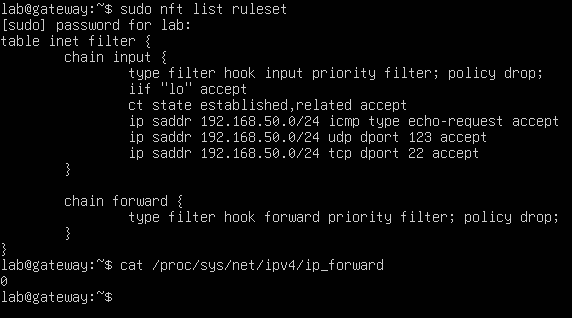
\includegraphics[width=0.58\linewidth]{fig/gateway-firewall-crop.png}\caption{Ruleset del gateway con \texttt{policy drop} e \texttt{ip\_forward = 0}.}\label{fig:gwfw}\end{figure}
\fig[0.95]{web-nginx-crop.png}{Servidor web: nginx activo y respuesta \texttt{HTTP/1.1 200 OK} (captura tomada durante el montaje, todavía con el adaptador NAT \texttt{enp0s3}).}
\fig[0.95]{dns-resolucion-crop.png}{DNS: \texttt{web.lab.local} resuelve a 192.168.50.20 en dnsmasq (captura del montaje, con NAT aún presente).}
\fig[0.95]{xmpp-prosody-crop.png}{XMPP: Prosody activo y escuchando en 5222 (IPv4 e IPv6).}
\fig[0.62]{web-ntp-crop.png}{Cliente NTP: la VM web sincroniza contra el gateway (\texttt{\^{}* 192.168.50.1}, \texttt{Reference ID C0A83201}).}
\begin{figure}[H]\centering
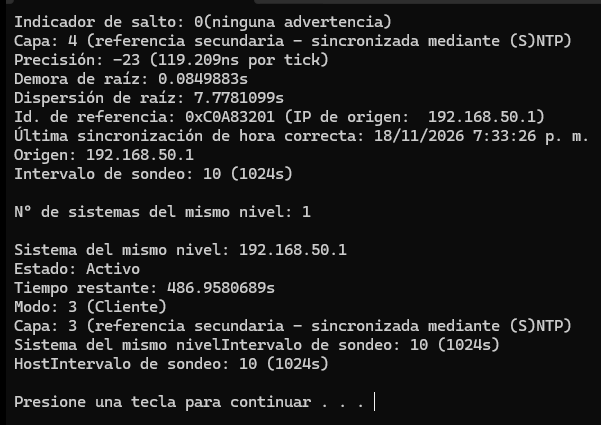
\includegraphics[width=0.48\linewidth]{fig/host-w32tm-crop.png}\hfill
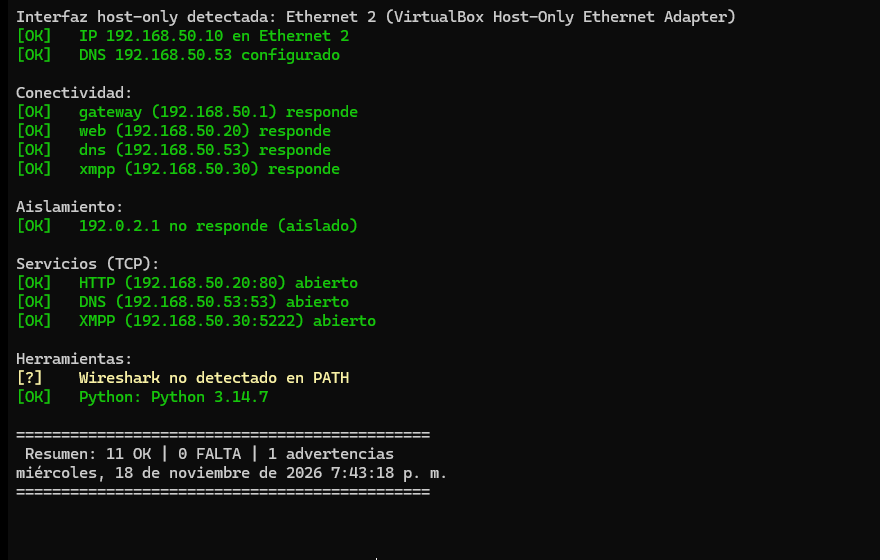
\includegraphics[width=0.48\linewidth]{fig/host-verificacion-analista-crop.png}
\caption{Analista Windows: w32time con origen 192.168.50.1 (izquierda) y verificación del rol analista con 11 OK, 0 FALTA y 1 advertencia (derecha).}\end{figure}
\fig{host-wireshark.png}{Captura en vivo en Wireshark sobre el adaptador \emph{Ethernet 2}: tráfico ICMP, TCP/HTTP, DNS y ARP del propio laboratorio.}

\section{Método de evidencia y reproducibilidad}\label{sec:metodo-evidencia}
\paragraph{Integridad.} Cada archivo se registra con SHA-256 (además de SHA-1 y MD5 por compatibilidad) en \cod{evidencia.log} con \cod{hash\_evidencia.py}. Al cerrar la Parte~I, \cod{scripts/cerrar\_parte\_i.py} copió 242 archivos a dos copias, \cod{original} y \cod{trabajo}, y generó un manifiesto JSON con ruta, tamaño y SHA-256 de cada uno, más la huella del propio manifiesto. La verificación recalcula todo y falla si un solo byte cambia.

\paragraph{Saltos de línea.} Git convirtió CRLF a LF los archivos de texto confirmados desde Windows, de modo que el manifiesto no verificaba en un clon. Se añadió \cod{.gitattributes} para guardar la evidencia byte a byte y \cod{scripts/reparar\_evidencia.py} restauró los CRLF originales. Cuatro archivos con saltos mixtos (\cod{caso03-auth-events}, \cod{caso03-ss-tulpn}, \cod{caso05-logs-correlacion} y \cod{caso06-openresolver}) no se podían reproducir; el manifiesto los registra en una lista de \emph{enmiendas} con su huella original, la actual y el motivo. Desde el commit \cod{02257d9} la verificación pasa en un clon limpio (Figura~\ref{fig:integridad}).

\paragraph{Reproducción.} Para este informe se clonó \cod{main} y se re-ejecutaron los analizadores sobre las mismas PCAP: las salidas de los casos 1, 2, 5, 6, 7 y 8 son idénticas byte a byte a las conservadas y las métricas del Caso~4 coinciden. Las capturas de terminal del capítulo~\ref{cap:parte1} provienen de esa re-ejecución.

\begin{figure}[H]\centering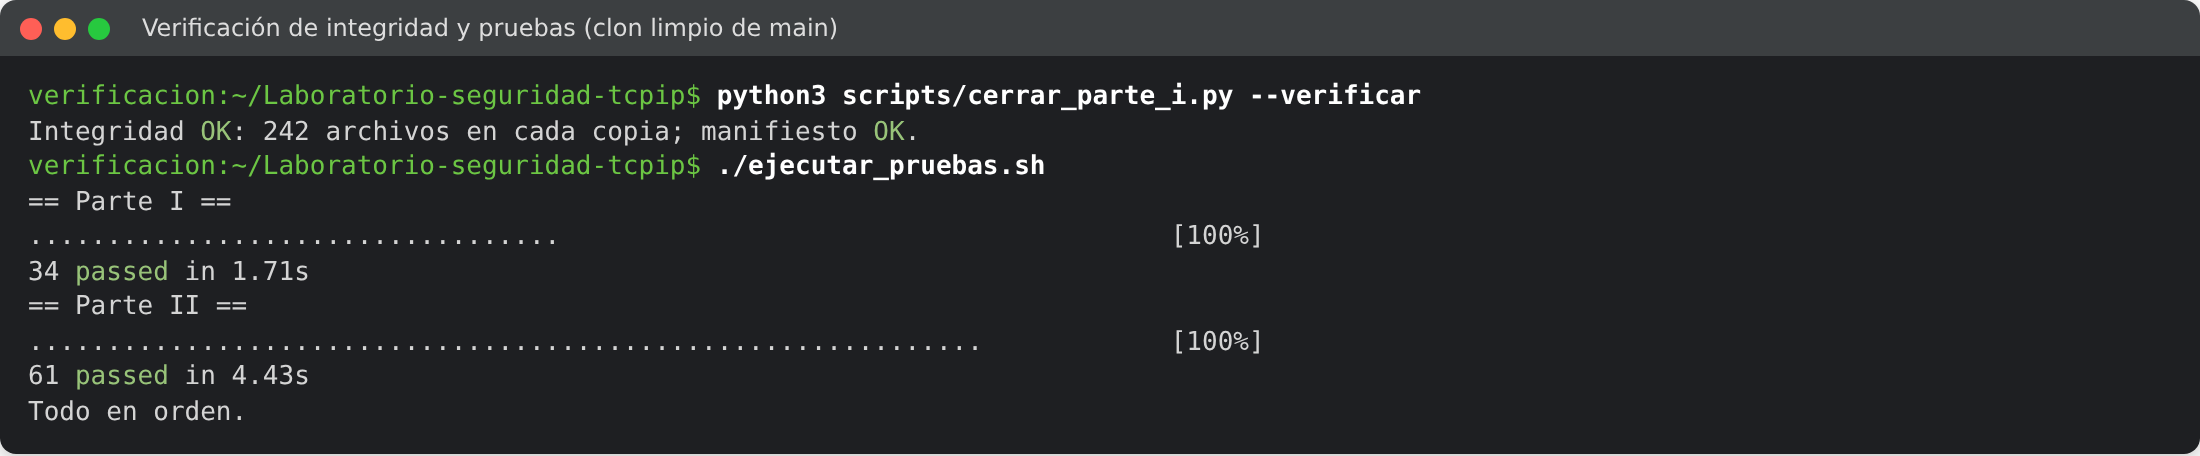
\includegraphics[width=\linewidth]{fig/term-integridad.png}
\caption{Verificación del manifiesto (242 archivos por copia) y ejecución de las pruebas de la Parte I (34) y la Parte II (61) en un clon limpio.}\label{fig:integridad}\end{figure}

\paragraph{Línea base.} \cod{baseline-normal.pcapng} (1.639 paquetes, 296,67~s) es tráfico real capturado en el analista, pero incluye ruido del propio Windows: consultas DNS a dominios externos, mDNS, LLMNR y NBNS. Se generó \cod{baseline-normal-limpia.pcapng} (720 paquetes, 293,26~s) conservando solo IPv4 dentro de 192.168.50.0/24 sin esos protocolos. La original se mantiene porque los casos cerrados verifican su huella; los casos 1, 4 y 7 se repitieron sobre la limpia (capítulo~\ref{cap:discusion}).

\fig{term-baseline.png}{Líneas base original y limpia: número de paquetes, duración y SHA-256.}

\section{Formato mínimo de registro por hallazgo}
Cada caso se documenta con una ficha de nueve campos. Como no se dispuso del apartado literal de la plantilla de la guía, se adoptó la estructura de la Tabla~\ref{tab:formato} y se declara como propuesta.

\begin{table}[H]\centering\small\caption{Campos de la ficha de registro por hallazgo.}\label{tab:formato}
\begin{tabularx}{\linewidth}{@{}p{3.2cm}X@{}}\toprule
\textbf{Campo} & \textbf{Contenido}\\\midrule
Identificador & Código del caso (CASO-01 a CASO-10)\\
Título & Hallazgo en una frase, sin afirmar más de lo demostrado\\
Fecha y analista & Fecha de ejecución y zona horaria; las marcas UTC se convierten a UTC$-$05:00\\
Categoría & Tipo de amenaza o técnica y si es estudio, simulación o incidente\\
Descripción & Qué se observó, con origen, destino y volúmenes\\
Severidad & Potencial y efectiva, separadas; criterio de impacto\\
Evidencias & Archivos con su huella en el manifiesto\\
Observables & Valores medidos que sostienen el hallazgo y el filtro usado\\
Estado & Qué queda confirmado y qué no; acciones pendientes\\
\bottomrule\end{tabularx}\end{table}

Además, cada caso incluye el procedimiento reproducible, la regla de detección o mitigación propuesta con su ubicación correcta en la red y preguntas de análisis.

\chapter{Parte I — Análisis de casos críticos}\label{cap:parte1}
Cada caso se documenta con su ficha de registro, el procedimiento y la evidencia analizada, la regla de detección o mitigación propuesta y las preguntas de análisis. Todos los PCAP de ataque son sintéticos: se generaron a archivo con direcciones privadas y no se enviaron a ninguna máquina. Las reglas nftables se validaron con \cod{nft -c -f} en el gateway (nftables 1.0.9, código de salida 0) sin aplicarlas: la validación comprueba la sintaxis, no la eficacia.

%======================================================================
\section{Caso 1 — TCP SYN flood: agotamiento de conexiones}
Un atacante que envía muchos SYN sin completar el saludo obliga al servidor a reservar estado para conexiones que nunca terminan. El caso modela una ráfaga contra el servidor web y el efecto de un limitador de tasa, y la compara con el tráfico HTTP real de la línea base.

\begin{ficha}{Ficha del Caso 1 — SYN flood.}
Identificador & CASO-01\\
Título & Ráfaga SYN sin handshake completo, modelada offline\\
Fecha y analista & 2026-11-18; análisis offline en el laboratorio autorizado\\
Categoría & Denegación de servicio TCP; simulación, no incidente\\
Descripción & 200 SYN de 192.168.50.100 a 192.168.50.20:80 en 10~s, más 3 conexiones HTTP completas. Un segundo PCAP modela un token bucket de 10/s con ráfaga 20 inicialmente lleno: pasan 120 SYN y se descartan 80, repartidos en toda la ráfaga\\
Severidad & Alta potencial (indisponibilidad del servicio); no se midieron recursos ni impacto real\\
Evidencias & \cod{caso01-synflood.pcap}, \cod{caso01-synflood-ratelimit.pcap}, \cod{caso01-analisis.txt}, \cod{caso01-syn-rate.png} (sintéticas); \cod{baseline-normal.pcapng} (real); \cod{caso01-regla.nft} (propuesta)\\
Observables & Sin filtro: SYN = 203, SYN-ACK = 203, ACK = 15, FIN = 6 (427 TCP). Con bucket: 123, 123, 15, 6 (267). 3 handshakes completos en ambos; 200 y 120 intentos sin completar. Pico de 20 SYN por ventana de 1~s\\
Estado & Patrón sintético confirmado; ataque real y eficacia de la mitigación no probados\\
\end{ficha}

\subsection{Procedimiento y evidencia}
\cod{gen\_caso01\_synflood.py} escribe ambas capturas y \cod{analizar\_caso01.py} las lee con \cod{tshark}. El analizador clasifica cada segmento en categorías excluyentes (RST, SYN-ACK, SYN, FIN, ACK restante) porque contar paquetes con bandera ACK mezclaría los SYN-ACK y los datos con el tercer paso del saludo. El handshake se correlaciona por \emph{stream}, 4-tupla, secuencia y reconocimiento \emph{raw}, orden temporal y un plazo de 10~s, descartando retransmisiones. Las tasas se calculan en ventanas de 1~s desde el inicio de la captura, incluidos los silencios.

\fig[0.98]{term-c01-tshark.png}{Primeros SYN del origen 192.168.50.100 hacia .20:80 en la captura sintética: puertos de origen consecutivos y ningún ACK posterior.}
\fig[0.98]{term-c01.png}{Salida de \texttt{analizar\_caso01.py}: categorías, handshakes correlacionados y comparación con la línea base real (0 SYN en 296,67~s).}
\fig{caso01-wireshark-final.png}{La captura sintética abierta en Wireshark por el grupo: ráfaga de SYN desde .100 y los SYN-ACK del servidor modelado.}
\fig[0.8]{caso01-syn-rate.png}{Arriba, SYN por ventana de 1~s en el modelo sin filtro y con token bucket: con ráfaga 20 el limitador deja pasar 20 en la primera ventana, así que 10/s no es un techo estricto por ventana aislada. Abajo, la línea base real de HTTP en .20: ningún SYN.}

La línea base real filtrada a HTTP de .20 tiene 57 segmentos TCP, 0 SYN y 0 handshakes: la captura empezó con sesiones ya abiertas. Eso no significa que no haya HTTP normal ni permite fijar un umbral de ``establecimientos normales''. La media de toda la captura sintética (9,67 SYN/s en 21~s) tampoco es la tasa de la ráfaga; hay que mirar las ventanas.

\subsection{Regla de detección y mitigación}
Tabla independiente para el host web .20, con política \emph{accept}, que solo descarta el exceso de SYN HTTP:
\begin{lstlisting}
table inet caso01_syn {
  chain input {
    type filter hook input priority 0; policy accept;
    ip daddr 192.168.50.20 tcp dport 80 tcp flags & (syn | ack) == syn \
      limit rate over 10/second burst 20 packets counter drop
  }
}
\end{lstlisting}
La palabra \cod{over} es esencial: sin ella la regla descartaría el tráfico \emph{dentro} del límite. El cubo es agregado, no por origen, de modo que un atacante también consumiría la cuota de los clientes legítimos. Debe instalarse en .20: el gateway no ve el tráfico directo entre peers de la subred.

\subsection{Mitigación}
\begin{itemize}
\item Activar SYN cookies en el servidor (\cod{net.ipv4.tcp\_syncookies = 1}) para no reservar estado hasta recibir el ACK.
\item Limitar la tasa de SYN por origen con conjuntos dinámicos de nftables (\cod{meter}) cuando haya un punto de filtrado en la ruta.
\item Ajustar el \emph{backlog} y los reintentos de SYN-ACK; en producción, apoyarse en el proveedor o en un balanceador con protección DoS.
\end{itemize}

\subsection{Preguntas de análisis}
\textbf{¿Basta contar paquetes con ACK para saber cuántas conexiones se completaron?} No. SYN-ACK y segmentos de datos también llevan ACK; hay que correlacionar el saludo por tupla y secuencia.\\
\textbf{¿Qué demuestra la segunda captura?} El comportamiento del modelo de token bucket, no que nftables filtró tráfico real ni que el servicio siguió disponible.\\
\textbf{¿Se puede inferir un umbral de ataque de esta línea base?} No: no contiene inicios de conexión HTTP.

%======================================================================
\section{Caso 2 — DNS tunneling: salida encubierta por UDP/53}
Un túnel DNS codifica datos en las etiquetas de los nombres consultados. El caso evalúa una heurística sencilla —longitud y entropía de Shannon de la etiqueta más larga— sobre consultas legítimas y artificiales.

\begin{ficha}{Ficha del Caso 2 — DNS tunneling.}
Identificador & CASO-02\\
Título & Longitud y entropía de la etiqueta DNS más larga\\
Fecha y analista & 2026-11-18; análisis offline\\
Categoría & Detección exploratoria de canal encubierto; datos sintéticos\\
Descripción & 37 consultas de .10 a .53: 12 nombres legibles del laboratorio y 25 con etiquetas hexadecimales aleatorias bajo \cod{exfil.lab.local}. No contienen datos robados\\
Severidad & Alta potencial (exfiltración); sin impacto comprobado\\
Evidencias & \cod{caso02-dns-tunneling.pcap}, \cod{caso02-analisis.txt}, \cod{caso02-dns-entropy.png} (sintéticas); \cod{caso02-dnsmasq-log.txt} (fragmento real)\\
Observables & Etiquetas hex de 25–52 caracteres con $H$ = 3,229–3,933 bits/símbolo; legibles de 5–7 caracteres con $H$ = 1,922–2,522; máximo 5 consultas hex por segundo\\
Estado & Heurística evaluada en muestra artificial; túnel y exfiltración no confirmados\\
\end{ficha}

\subsection{Procedimiento y evidencia}
El analizador filtra consultas (\cod{dns.flags.response == 0}), normaliza el nombre a minúsculas, toma la etiqueta más larga y calcula su longitud y su entropía
\[ H = -\sum_{c} p(c)\,\log_2 p(c), \]
donde $p(c)$ es la frecuencia relativa de cada carácter. En hexadecimal $H$ no puede pasar de 4 bits. La regla propuesta es \emph{longitud $>$ 30 o $H >$ 3,5}.

\fig[0.98]{term-c02-tshark.png}{Consultas del PCAP: nombres legibles del laboratorio seguidos de la tanda de etiquetas hexadecimales bajo \texttt{exfil.lab.local}.}
\fig[0.98]{term-c02.png}{Salida de \texttt{analizar\_caso02.py}: agrupación por origen y sufijo, 21 de 25 nombres artificiales marcados y 0 de 12 legibles, y la consulta real del log de dnsmasq.}
\fig{caso02-wireshark-final.png}{Las consultas sintéticas en Wireshark.}
\fig[0.75]{caso02-dns-entropy.png}{Longitud frente a entropía de la etiqueta más larga: los nombres legibles quedan abajo a la izquierda; cuatro artificiales cortos no superan ningún umbral.}

La regla marca 21 de 25 nombres artificiales y ninguno legible: no separa perfectamente. Los cuatro que no marca son etiquetas cortas cuya entropía queda bajo 3,5; no por eso son benignos. El log real de dnsmasq conserva una consulta demostrativa (etiqueta de 52 caracteres, $H$ = 3,724) hecha desde .53, no desde .10: coincide en el nombre pero no hay correspondencia de tiempos ni transacciones con la tanda sintética, y la respuesta fue REFUSED. No prueba ningún canal.

\subsection{Reglas de detección y mitigación}
La detección se implementa en Python, no como firma de IDS: se retiró una pseudofirma con \cod{byte\_test} sobre \cod{dns.query} porque ese búfer contiene el nombre ya normalizado, sin los octetos de longitud del formato de red. Para un IDS se propone, como señal de revisión y no de bloqueo:
\begin{itemize}
\item contar por cliente y dominio base las consultas con etiqueta $>$ 30 caracteres o $H >$ 3,5 en ventanas de 60~s, y alertar por volumen sostenido;
\item vigilar respuestas TXT o NULL grandes y frecuentes hacia un mismo dominio.
\end{itemize}

\subsection{Mitigación}
\begin{itemize}
\item Forzar que los clientes solo usen el resolver interno (.53) y bloquear DNS saliente directo en el punto de salida.
\item Activar el registro de consultas en el resolver y revisar dominios con muchas etiquetas únicas.
\item Usar listas de bloqueo o RPZ para dominios conocidos de túnel; no bloquear solo por entropía sin validar falsos positivos.
\end{itemize}

\subsection{Preguntas de análisis}
\textbf{¿Qué mide la entropía?} La diversidad de símbolos de la etiqueta, no la intención: un CDN o un identificador aleatorio legítimo también la eleva.\\
\textbf{¿Qué confirma el log real?} Una consulta demostrativa desde .53, no la ejecución del escenario sintético ni una exfiltración.\\
\textbf{¿Puede reutilizarse el umbral?} Como señal exploratoria, hasta calibrarlo con tráfico real.

%======================================================================
\section{Caso 3 — Exposición de servicios HTTP, FTP y heredados}
Cada servicio en escucha es una puerta posible. El caso levanta el inventario real de sockets de las cuatro VMs y del anfitrión y valora su riesgo.

\begin{ficha}{Ficha del Caso 3 — Servicios expuestos.}
Identificador & CASO-03\\
Título & Inventario de sockets en escucha; accesibilidad efectiva pendiente\\
Fecha y analista & 2026-11-18; laboratorio autorizado\\
Categoría & Endurecimiento e inventario; no intrusión\\
Descripción & \cod{ss -tulpn} observa SSH en las cuatro VMs, HTTP en web, DNS en .53, NTP en el gateway y XMPP 5222/5269 en .30. \cod{netstat} del anfitrión observa además 139, 445 y 5432. No hay FTP ni Telnet en ninguna VM\\
Severidad & Media provisional, según necesidad y alcance real de cada servicio\\
Evidencias & \cod{caso03-ss-tulpn.txt}, \cod{caso03-netstat-host.txt}, \cod{caso03-auth-events.txt}, \cod{caso03-netstat-consola.png} (reales); \cod{caso03-riesgo.png} (valoración)\\
Observables & Sockets de la Tabla~\ref{tab:inventario}; en los fragmentos de autenticación, 8 \cod{Accepted password} y 0 \cod{Failed password}\\
Estado & Inventario observado; necesidad y accesibilidad remota no verificadas; sin evidencia de intrusión\\
\end{ficha}

\begin{table}[H]\centering\small\caption{Inventario observado de servicios en escucha.}\label{tab:inventario}
\begin{tabularx}{\linewidth}{@{}p{2.4cm}p{5.2cm}X@{}}\toprule
\textbf{Equipo} & \textbf{Escucha observada} & \textbf{Atribución y alcance}\\\midrule
gateway .1 & TCP 22 IPv4/IPv6; UDP 123 IPv4 & sshd, chronyd\\
web .20 & TCP 22 y 80 IPv4/IPv6 & sshd, nginx\\
dns .53 & TCP/UDP 53 en .53; TCP 22 & dnsmasq, sshd\\
xmpp .30 & TCP 22, 5222, 5269 IPv4/IPv6 & sshd, Prosody (lua5.4)\\
VMs & 53 y 323 en loopback & resolvedor y chrony locales; sin acceso remoto\\
anfitrión & TCP 139 en tres interfaces; 445 en todas & PID 4 (sistema); proceso no atribuido\\
anfitrión & TCP 5432 en todas & PID 6404; proceso no atribuido\\
\bottomrule\end{tabularx}\end{table}

\subsection{Procedimiento y evidencia}
\fig[0.98]{term-c03.png}{Salida de \texttt{analizar\_caso03.py}: sockets del anfitrión con su PID y conteo de eventos de autenticación.}
\fig{caso03-netstat-consola.png}{Consola del analista con el inventario original (el rótulo heredado ``Conexiones establecidas'' no filtra por estado: incluye LISTENING y TIME\_WAIT).}
\fig[0.8]{caso03-riesgo.png}{Valoración cualitativa propuesta de impacto y probabilidad por servicio; no es un riesgo medido.}

Que un puerto escuche no prueba que sea alcanzable desde otro equipo: intervienen la ruta, el firewall local y las ACL del servicio. Tampoco se identifica un producto solo por el número de puerto: 445 suele ser SMB y 5432 PostgreSQL, pero el PID registrado no se correlacionó con su proceso en el instante de la captura. Cero \cod{Failed password} en un fragmento no demuestra ausencia de intentos fallidos en todo el periodo.

\subsection{Plan de endurecimiento}
\begin{itemize}
\item Restringir SSH en cada VM a orígenes autorizados (incluido IPv6) y exigir llaves en lugar de contraseña.
\item Evaluar si hace falta federación XMPP (5269); si no, cerrarla en .30, no en el gateway.
\item Auditar en el anfitrión qué proceso ocupa 139/445/5432 y si debe escuchar en todas las interfaces.
\item Revisar que dnsmasq no responda recursión a orígenes no autorizados (ver Caso~6) y considerar TLS para HTTP según los datos que transporte.
\item Verificar el alcance con pruebas benignas autorizadas antes de cerrar servicios.
\end{itemize}

\subsection{Preguntas de análisis}
\textbf{¿Escuchar implica exposición remota?} No: depende de la ruta, el firewall y las ACL.\\
\textbf{¿Dónde se filtra el tráfico entre peers?} En cada equipo, o en un dispositivo que realmente esté en su camino.\\
\textbf{¿Qué significa no ver \texttt{Failed password}?} Solo que no aparece en estos fragmentos.

%======================================================================
\section{Caso 4 — Detección de anomalías con IA/ML en tráfico TCP/IP}
El caso evalúa con método dos detectores no supervisados —z-score e Isolation Forest— entrenados con la línea base real y probados con ventanas normales posteriores y con anomalías sintéticas. Una primera versión con 28 ventanas de duración desigual, etiquetas por PCAP y evaluación sobre los mismos datos de entrenamiento se declaró obsoleta y se rehízo.

\begin{ficha}{Ficha del Caso 4 — Anomalías con ML.}
Identificador & CASO-04\\
Título & Evaluación temporal de z-score e Isolation Forest con normales reales y anomalías tabulares sintéticas\\
Fecha y analista & 2026-11-18 (ejecuciones fechadas en UTC 2026-11-19)\\
Categoría & Evaluación metodológica de detección no supervisada\\
Descripción & 29 ventanas completas de 10~s: 17 de entrenamiento, 1 de embargo, 11 de prueba normal; 22 variantes sintéticas (11 SYN y 11 DNS) construidas sobre ventanas de prueba\\
Severidad & Media metodológica; no es un incidente\\
Evidencias & \cod{scripts/caso04\_ml.py}; \cod{caso04-dataset.csv}, \cod{caso04-metricas.json}, \cod{caso04-predicciones.csv}, \cod{caso04-manifiesto.json}, gráficas\\
Observables & Ambos detectores marcan 22/22 sintéticas. Falsos positivos sobre normales: z-score 1/11 (FPR 0,091), Isolation Forest 5/11 (FPR 0,455). 19 autopruebas aprobadas\\
Estado & Exploratorio: muestra pequeña, una sola captura y ninguna anomalía real de prueba\\
\end{ficha}

\subsection{Atributos y separación temporal}
Se extraen 30 atributos por ventana de 10~s: volumen y flujos (paquetes, bytes, flujos, puertos destino), duración de flujos dentro de la ventana, tasas, banderas TCP y sus proporciones, intentos SYN deduplicados, pares petición/respuesta DNS y HTTP, y longitud media de los nombres consultados. Las etiquetas, IP, sufijos y marcas de tiempo quedan fuera de los atributos para que el modelo no ``haga trampa''.

\begin{table}[H]\centering\small\caption{Particiones del Caso 4.}
\begin{tabularx}{\linewidth}{@{}llX@{}}\toprule
\textbf{Partición} & \textbf{Ventanas} & \textbf{Uso}\\\midrule
Entrenamiento & 0–16 (17), [0,170)~s & Único ajuste de media, desviación y árboles\\
Embargo & 17 (1), [170,180)~s & Ni entrena ni evalúa: reduce la autocorrelación\\
Prueba normal & 18–28 (11), [180,290)~s & Falsos positivos sobre normales posteriores\\
Prueba sintética & 11 SYN + 11 DNS & Sensibilidad; padres solo de prueba\\
\bottomrule\end{tabularx}\end{table}

Cada variante conserva el fondo completo de una ventana de prueba e inserta registros sintéticos entre los segundos 2 y 8, con semilla 42. Son filas de una tabla, no paquetes transmitidos. El z-score alerta si algún atributo no constante supera $|z| > 3$ con media y desviación del entrenamiento; Isolation Forest usa 200 árboles, \cod{contamination=auto} y umbral nativo.

\subsection{Resultado de los detectores}
\fig[0.98]{term-c04.png}{Salida de \texttt{caso04\_ml.py}: huella de la línea base, particiones y matrices de confusión solo sobre prueba (filas = etiqueta, columnas = predicción).}

\begin{table}[H]\centering\small\caption{Métricas del Caso 4 sobre prueba.}
\begin{tabular}{@{}lcccc@{}}\toprule
\textbf{Conjunto} & \multicolumn{2}{c}{\textbf{z-score}} & \multicolumn{2}{c}{\textbf{Isolation Forest}}\\
 & Acierto & FPR & Acierto & FPR\\\midrule
Normales reales (11) & 10/11 & 0,091 & 6/11 & 0,455\\
SYN sintéticas (11) & 11/11 & — & 11/11 & —\\
DNS sintéticas (11) & 11/11 & — & 11/11 & —\\
Mezcla didáctica (33) & F1 0,978 & 0,091 & F1 0,898 & 0,455\\
\bottomrule\end{tabular}\end{table}

\fig[0.9]{caso04-matriz-confusion.png}{Matrices de confusión de ambos detectores sobre el conjunto mixto de prueba.}
\fig[0.8]{caso04-scatter.png}{Ventanas en dos atributos: las variantes sintéticas se alejan claramente de las normales, lo que explica la detección perfecta y advierte que la tarea es fácil.}
\fig{caso04-consola-revisada.png}{Ejecución del experimento revisado en el equipo analista.}

\subsection{Interpretación y uso responsable}
Detectar 22 de 22 no prueba capacidad real: las anomalías sintéticas son grandes y comparten fondo con su ventana padre, así que no aumentan el tamaño efectivo de la muestra. Lo informativo son los falsos positivos: Isolation Forest marca casi la mitad de las ventanas normales posteriores, lo que en operación saturaría al analista. Al repetir con la línea base limpia, el falso positivo del z-score desaparece (capítulo~\ref{cap:discusion}). Un modelo así sirve para ordenar qué revisar primero, no para bloquear automáticamente.

\subsection{Preguntas de análisis}
\textbf{¿Por qué separar en el tiempo?} Ventanas vecinas se parecen; mezclarlas entre entrenamiento y prueba infla las métricas.\\
\textbf{¿Cuál detector es mejor?} Con una captura y 11 normales no hay base para una comparación fuerte; el z-score tuvo menos falsos positivos en este conjunto.\\
\textbf{¿Qué haría falta?} Varias capturas de días distintos, anomalías reales etiquetadas por humanos y calibración del umbral en un conjunto de validación independiente.

%======================================================================
\section{Caso 5 — TCP: resets inesperados e indicios de inyección}
Un RST con la tupla y la secuencia correctas puede cortar una sesión ajena. El caso distingue RST dentro de sesiones observadas de RST sueltos.

\begin{ficha}{Ficha del Caso 5 — Resets TCP.}
Identificador & CASO-05\\
Título & RST en sesiones modeladas y cuatro RST fuera de flujo\\
Fecha y analista & 2026-11-18; análisis offline\\
Categoría & Análisis TCP; no inyección demostrada\\
Descripción & 6 RST: uno del servidor .20:80 a .10:31000, uno del cliente .10:32000 a .30:5222 y cuatro de .100:41000–41003 a .20:80 sin sesión previa\\
Severidad & Media potencial (interrupción de sesiones); ninguna sesión real interrumpida\\
Evidencias & \cod{caso05-rst.pcap}, \cod{caso05-analisis.txt} (sintéticas); \cod{caso05-logs-correlacion.txt} (fragmentos reales de nginx y Prosody)\\
Observables & 2 RST con handshake previo y 4 fuera de flujo; secuencias \emph{raw} 400000, 400100, 400200 y 400300; ack = 0 y bandera ACK ausente\\
Estado & Casos sintéticos; ni ataque ni falsificación confirmados\\
\end{ficha}

\subsection{Procedimiento y evidencia}
El analizador filtra \cod{tcp.flags.reset == 1} y para cada RST busca un saludo previo con la misma 4-tupla, usando los números de secuencia \emph{raw} (Wireshark muestra secuencias relativas por defecto).

\fig[0.98]{term-c05.png}{Salida de \texttt{analizar\_caso05.py} y lista de RST con secuencias \emph{raw}: los cuatro de .100 usan tuplas sin sesión previa.}
\fig{caso05-wireshark-final.png}{Los RST en Wireshark con \texttt{tcp.relative\_sequence\_numbers:FALSE} solo para esa vista.}

Los cuatro RST de .100 no comparten la 4-tupla de ninguna sesión: son RST fuera de flujo, no resets efectivos de una conexión ajena. Un RST sin bandera ACK es legal (por ejemplo, respuesta a un segmento hacia un puerto sin sesión), y con ACK apagado el campo ack no tiene significado: \emph{ack = 0} no prueba suplantación. Los logs reales de nginx y Prosody son de otra hora y no se correlacionan con este PCAP generado.

\subsection{Regla de detección propuesta}
Se retiró una pseudofirma que equiparaba \cod{ack:0} con RST forjado. Se propone, como señal de revisión, contar RST por origen sin sesión previa en ventanas cortas y enriquecer con el estado de la conexión y la ventana de secuencia aceptable antes de atribuir intención.

\subsection{Mitigación}
\begin{itemize}
\item Mantener las pilas TCP actualizadas: RFC 5961 \cite{rfc5961} exige que un RST esté exactamente en la secuencia esperada o responder con un \emph{challenge ACK}.
\item Cifrar y autenticar las aplicaciones (TLS) para que un corte no permita inyectar datos.
\item Filtrado de origen en el acceso para dificultar la suplantación.
\end{itemize}

\subsection{Preguntas de análisis}
\textbf{¿Son inyección los RST de .100?} No en una sesión observada: usan otras tuplas.\\
\textbf{¿Basta \emph{ack = 0} para alertar?} No; un RST sin ACK es legítimo en varios contextos.\\
\textbf{¿Qué haría falta para correlacionar?} Captura y logs de la misma ejecución, con sesiones identificables y evidencia del endpoint.

%======================================================================
\section{Caso 6 — UDP: reflexión y amplificación DNS, NTP o SSDP}
En la reflexión, el atacante envía solicitudes pequeñas con la IP de la víctima falsificada a un servicio que responde con mucho más tráfico. El caso modela esa asimetría con datagramas genéricos y comprueba con una consulta real si el resolver del laboratorio responde a recursión.

\begin{ficha}{Ficha del Caso 6 — Reflexión UDP.}
Identificador & CASO-06\\
Título & Modelo de reflexión con datagramas genéricos, no un amplificador NTP real\\
Fecha y analista & 2026-11-18; análisis offline y una consulta real benigna\\
Categoría & Denegación de servicio reflectiva; simulación\\
Descripción & 20 pares entre .20:52000–52019 y .200:40000 con payloads de 48 y 468~B; el guion asigna la MAC de .100 a solicitudes con IP .20 (suplantación modelada). Incluye un par DNS válido \cod{web.lab.local} entre .10 y .53\\
Severidad & Alta potencial; no se midió saturación ni amplificación de un servicio real\\
Evidencias & \cod{caso06-reflexion-udp.pcap}, \cod{caso06-analisis.txt}, \cod{caso06-udp-rate.png} (sintéticas); \cod{caso06-openresolver-revision.txt} (real); \cod{caso06-openresolver.txt} (real, histórico incompleto)\\
Observables & 42 datagramas; sin DNS: 1800~B de tramas de solicitud y 10200~B de respuesta (5,667x); payload 960 frente a 9360~B (9,750x). Consulta real: REFUSED\\
Estado & Asimetría sintética calculada; reflector real no probado\\
\end{ficha}

\subsection{Procedimiento y evidencia}
El factor de amplificación se define como
\[ \text{BAF} = \frac{\text{bytes de respuesta}}{\text{bytes de solicitud}}, \]
y se informa tanto sobre tramas capturadas (sin FCS ni relleno Ethernet) como sobre payload UDP. Las tasas se normalizan por el ancho nominal de ventana de 0,5~s.

\fig[0.98]{term-c06-tshark.png}{Primeros datagramas del PCAP: el par DNS válido y las solicitudes de 48~B seguidas de respuestas de 468~B en el puerto 40000.}
\fig[0.98]{term-c06.png}{Salida de \texttt{analizar\_caso06.py}: cocientes de amplificación, tasas por ventana y la prueba real de resolver abierto.}
\fig{caso06-wireshark-final.png}{El modelo UDP y el DNS válido en Wireshark; el puerto 40000 no se presenta como NTP.}
\fig[0.75]{caso06-udp-rate.png}{Paquetes y bytes por segundo normalizados por ventana de 0,5~s; la última ventana está observada solo en parte.}

En la ventana [1,0;1,5)~s hay 25 datagramas (50 paquetes/s y 8700~B/s) y en [1,5;2,0)~s, 15 datagramas (30 paquetes/s y 15300~B/s): pocas respuestas grandes pesan más que muchas solicitudes pequeñas. El cociente diseñado no mide la amplificación de ningún servicio real; como referencia, la literatura reporta factores mucho mayores para NTP \emph{monlist}, DNS abierto o SSDP \cite{rossow2014}.

\paragraph{Prueba real de resolver abierto.} Desde .53 se consultó \cod{dig -b 192.168.50.53 @192.168.50.53 example.com A +time=2 +tries=1} (2026-11-18 20:47:31 $-$05): respuesta \textbf{REFUSED} con EDE~14 (\emph{Not Ready}), 46~B, código de salida 0. dnsmasq, configurado con \cod{no-resolv}, no resuelve nombres externos. Solo prueba el rechazo de esa consulta, origen e instante, no la ausencia universal de reflectores. El archivo histórico perdió su stderr y se conserva sin completarlo.

\subsection{Mitigación}
\begin{itemize}
\item Desactivar la recursión abierta en resolvers y restringirla por ACL; aplicar \emph{Response Rate Limiting}.
\item En NTP, deshabilitar comandos de control como \emph{monlist}; en SSDP, no exponer UPnP fuera de la LAN.
\item Filtrado de origen (BCP~38 \cite{bcp38}) en el acceso para impedir paquetes con IP de origen ajena; en una misma subred hace falta protección en el switch (por ejemplo, \emph{IP source guard}).
\end{itemize}

\subsection{Preguntas de análisis}
\textbf{¿El cociente prueba amplificación NTP?} No: son payloads genéricos diseñados.\\
\textbf{¿Qué prueba REFUSED?} Que esa consulta concreta fue rechazada, nada universal.\\
\textbf{¿Cómo comparar tasas?} Dividiendo por el ancho de ventana y declarando las ventanas parciales.

%======================================================================
\section{Caso 7 — ICMP: escaneo, payloads atípicos y posible túnel}
ICMP sirve para diagnosticar, pero ráfagas de echo o cargas grandes pueden indicar reconocimiento o un canal encubierto. El caso compara un escenario sintético con el ICMP real de la línea base.

\begin{ficha}{Ficha del Caso 7 — ICMP.}
Identificador & CASO-07\\
Título & Tamaños y frecuencias de ICMP echo sintético frente a la línea base real\\
Fecha y analista & 2026-11-18; análisis offline\\
Categoría & Señales exploratorias de tamaño y frecuencia; no exfiltración\\
Descripción & 63 paquetes: cuatro pares request/reply de .10 con las VMs, 50 requests de .100 a .20 con 64~B y cinco requests con 1289~B de datos\\
Severidad & Media-alta potencial; sin degradación ni canal demostrados\\
Evidencias & \cod{caso07-icmp.pcap}, \cod{caso07-analisis.txt}, \cod{caso07-icmp-freq.png} (sintéticas); \cod{baseline-normal.pcapng} (real); \cod{caso07-regla-icmp.nft} (propuesta)\\
Observables & .100 emite 55 echo, máximo 10 por ventana de 1~s; payloads 9/64/1289~B (tramas 51/106/1331~B). Línea base: 152 echo de 32~B, máximo 1/s, ninguno $>$ 200~B\\
Estado & Diferencias observadas en simulación; túnel y umbrales no confirmados\\
\end{ficha}

\subsection{Procedimiento y evidencia}
Se leen ambas capturas filtrando echo IPv4 (tipos 0 y 8) sin fragmentar. El payload se calcula como \cod{ip.len - ip.hdr\_len - 8}, no con \cod{frame.len}, que incluye las cabeceras Ethernet, IPv4 e ICMP.

\fig[0.98]{term-c07.png}{Salida de \texttt{analizar\_caso07.py} y paquetes de .100: requests de 64~B cada 0,1~s y cinco de 1289~B de datos (1331~B de trama).}
\fig{caso07-wireshark-final.png}{El escenario ICMP en Wireshark.}
\fig[0.8]{caso07-icmp-freq.png}{Echo-request por ventana de 1~s y por origen en el modelo (arriba: .100 sostiene 10/s) y en la línea base real (abajo: .10 hace ping a las cuatro VMs aproximadamente cada 15~s), cada uno con su eje temporal.}

En la línea base real, .10 hace ping a cada VM cada 15~s aproximadamente: 19 requests en 296,67~s (0,064/s) con 32~B, el tamaño por defecto de \cod{ping} en Windows. El modelo alcanza 10/s y cinco cargas de 1289~B, valores que destacan frente a esa referencia; pero un ping con \cod{-l 1300} legítimo produce lo mismo.

\subsection{Regla de detección y mitigación}
Para el host web .20: descartar solo el exceso de echo-request.
\begin{lstlisting}
table inet caso07_echo {
  chain input {
    type filter hook input priority 0; policy accept;
    ip daddr 192.168.50.20 icmp type echo-request \
      limit rate over 5/second burst 10 packets counter drop
  }
}
\end{lstlisting}
Como detección, alertar (sin bloquear) cuando un origen supere 5 echo/s sostenidos o envíe payloads mayores a 200~B, umbrales propuestos que requieren calibración.

\subsection{Mitigación}
\begin{itemize}
\item Limitar la tasa de echo por host y permitir los tipos ICMP necesarios para la red (\emph{destination unreachable}, \emph{fragmentation needed}); bloquear todo ICMP rompe el descubrimiento de MTU.
\item Para canales encubiertos, inspeccionar la entropía y la variación del contenido de los payloads, además del tamaño.
\end{itemize}

\subsection{Preguntas de análisis}
\textbf{¿1331~B es el payload?} No: son 1289~B de datos más cabeceras.\\
\textbf{¿Un paquete grande prueba un túnel?} No; hay diagnósticos legítimos con payloads grandes.\\
\textbf{¿Qué aporta la línea base?} Una referencia medida y acotada, no una regla universal.

%======================================================================
\section{Caso 8 — Escaneo de puertos y fingerprinting de servicios}
El reconocimiento suele preceder a un ataque. La señal de un escaneo no es el número de paquetes sino cuántos puertos \emph{distintos} sondea un origen en poco tiempo.

\begin{ficha}{Ficha del Caso 8 — Escaneo de puertos.}
Identificador & CASO-08\\
Título & Sondeos SYN sintéticos y lista parcial de respuestas programadas\\
Fecha y analista & 2026-11-18; análisis offline\\
Categoría & Reconocimiento TCP; no descubrimiento real\\
Descripción & .100 envía 25 SYN: 20 a .20 y 5 a .30. Son 24 números de puerto únicos porque el 80 se sondea en ambos destinos\\
Severidad & Media potencial; sin impacto\\
Evidencias & \cod{caso08-portscan.pcap}, \cod{caso08-analisis.txt}, \cod{caso08-portscan.png} (sintéticas); \cod{caso08-regla-portscan.nft} (propuesta)\\
Observables & 25 SYN, 21 RST y 4 SYN-ACK programados (.20:22 y 80; .30:5222 y 5269); ningún handshake completo\\
Estado & Patrón sintético; exposición real no confirmada\\
\end{ficha}

\subsection{Procedimiento y evidencia}
Se filtran SYN iniciales (\cod{tcp.flags.syn == 1 \&\& tcp.flags.ack == 0}) y se calcula, por ventana fija, origen y destino, el número de SYN y la cardinalidad del conjunto de puertos.

\fig[0.98]{term-c08-tshark.png}{Sondeo secuencial de .100 a .20: un SYN por puerto y la respuesta RST o SYN-ACK programada.}
\fig[0.98]{term-c08.png}{Salida de \texttt{analizar\_caso08.py}: 20 puertos distintos hacia .20 en menos de 0,2~s y 5 hacia .30.}
\fig{caso08-wireshark-final.png}{El escaneo en Wireshark.}
\fig[0.75]{caso08-portscan.png}{Puertos destino distintos por origen y destino en la ventana [0,1)~s: 20 hacia .20 y 5 hacia .30.}

La lista de respuestas es parcial y escrita en el generador: no incluye SSH de .30, aunque ese puerto sí escucha según el inventario real del Caso~3. Coincidir parcialmente con el inventario no significa que se descubrió nada.

\subsection{Regla de detección y mitigación}
Registro limitado de SYN en los endpoints .20 y .30, sin descartar:
\begin{lstlisting}
table inet caso08_observacion {
  chain input {
    type filter hook input priority 0; policy accept;
    ip daddr { 192.168.50.20, 192.168.50.30 } tcp flags & (syn | ack) == syn \
      limit rate 5/second burst 10 packets log prefix "scan-syn: " counter
  }
}
\end{lstlisting}
El \cod{limit} antes de \cod{log} limita la escritura de registros, así que el log pierde eventos y no sirve para contar cardinalidad; esta se calcula sobre el PCAP completo. Criterio de revisión propuesto: 20 o más puertos distintos por origen y destino en 1~s.

\subsection{Plan de endurecimiento}
\begin{itemize}
\item Cerrar lo innecesario y filtrar por origen en cada host (política \emph{drop} con excepciones explícitas).
\item Ocultar banners de versión en servicios (nginx \cod{server\_tokens off}) para dificultar el \emph{fingerprinting}.
\item Usar conjuntos dinámicos de nftables para registrar orígenes que tocan muchos puertos distintos.
\end{itemize}

\subsection{Preguntas de análisis}
\textbf{¿25 SYN son 25 puertos únicos?} No: el 80 se repite entre destinos, y las retransmisiones inflan el conteo sin aumentar la cardinalidad.\\
\textbf{¿Un SYN-ACK del PCAP confirma un puerto abierto real?} No, está programado.\\
\textbf{¿El \texttt{limit} del log detecta escaneos?} No; solo controla el volumen de registros.

%======================================================================
\section{Caso 9 — Priorización y correlación de alertas con IA y SIEM}\label{sec:caso9}
Una alerta aislada rara vez basta. El caso construye un pipeline local que normaliza logs reales del laboratorio, los agrupa por origen y minuto, y asigna un puntaje explicable. Como no se instaló Wazuh, el pipeline en Python cumple sus etapas: recolección, normalización, correlación, puntuación y presentación.

\begin{ficha}{Ficha del Caso 9 — Correlación SIEM.}
Identificador & CASO-09\\
Título & Correlación de logs con puntaje explicable\\
Fecha y analista & 2026-11-18; revisión humana pendiente\\
Categoría & Detección por origen y ventana de 60~s\\
Descripción & 168 eventos reales normalizados (auth, nginx, Prosody y dnsmasq; el fragmento real de nftables no tenía registros) y 21 registros sintéticos forman 37 ventanas; 0 alertas reales y 1 sintética de 49 puntos\\
Severidad & Alta para el escenario didáctico; no hay incidente real\\
Evidencias & \cod{caso09-logs/}, \cod{caso09-eventos-normalizados.csv}, \cod{caso09-escenario-sintetico.jsonl}, \cod{caso09-alertas.json}, \cod{caso09-scores.txt}, \cod{caso09-cobertura.json}\\
Observables & Origen sintético 192.168.50.100: 6 fallos de autenticación, 3 errores HTTP 5xx y 12 puertos distintos en un minuto, en auth, nginx y nftables\\
Estado & Pipeline probado automáticamente; dictamen humano pendiente en \cod{caso09-validacion-humana.json}\\
\end{ficha}

\subsection{Etapas del pipeline}
\fig{caso09-pipeline.png}{Etapas del pipeline de correlación local.}
\begin{table}[H]\centering\small\caption{Etapas del pipeline del Caso 9.}
\begin{tabularx}{\linewidth}{@{}p{2.8cm}X@{}}\toprule
\textbf{Etapa} & \textbf{Qué hace}\\\midrule
Recolección & Lee fragmentos exportados de cada VM; guarda archivo, línea y SHA-256 de cada registro\\
Normalización & Esquema común: tiempo UTC, fuente, host que informa, origen observado, tipo de evento. Los syslog sin año ni zona se interpretan como 2026 y UTC$-$05:00, supuesto declarado\\
Correlación & Agrupa por procedencia (real o sintética), IP de origen y minuto; si el log no trae origen queda ``no atribuido'', nunca se toma la IP de otra línea\\
Puntuación & Suma reglas explicables (Tabla~\ref{tab:prio})\\
Presentación & Alerta con factores, fuentes, hosts y referencias a las líneas originales; recomienda revisar, no bloquea\\
\bottomrule\end{tabularx}\end{table}

\subsection{Criterios de prioridad}
\begin{table}[H]\centering\small\caption{Reglas de puntuación (umbral de alerta: 10 puntos por ventana).}\label{tab:prio}
\begin{tabular}{@{}lll@{}}\toprule
\textbf{Indicador} & \textbf{Condición} & \textbf{Puntos}\\\midrule
Fallos de autenticación & $\geq 3$ en la ventana & 5 por evento\\
Errores HTTP 5xx & $\geq 3$ & 3 por evento\\
Puertos destino distintos en SYN & $\geq 10$ & 10\\
Consultas DNS con etiqueta $>$ 30 & $\geq 3$ & 6\\
\bottomrule\end{tabular}\end{table}

\subsection{Ejemplo de alerta enriquecida}
\fig[0.98]{term-c09.png}{Re-ejecución del pipeline: 168 eventos reales, 21 sintéticos, 37 ventanas, 0 alertas reales y 1 sintética.}
\begin{lstlisting}
{ "evidence_kind": "sintetica", "subject": "192.168.50.100",
  "window_utc": "2026-11-19T01:30:00+00:00", "window_seconds": 60,
  "reporting_hosts": ["gateway", "web"], "sources": ["auth", "nftables", "nginx"],
  "counts": {"AUTH_FAIL": 6, "HTTP_5XX": 3, "NFT_SYN": 12},
  "distinct_dst_ports": 12, "score": 49,
  "factors": {"fallos_autenticacion": 30, "errores_http_5xx": 9,
              "diez_puertos_distintos": 10},
  "alert": true, "evidence_refs": ["caso09-escenario-sintetico.jsonl:1", ...] }
\end{lstlisting}
El puntaje se explica solo: 30 + 9 + 10 = 49. El escenario de las 20:30 locales corresponde a las 01:30 UTC del 19 de noviembre.
\fig{caso09-consola-final.png}{Ejecución del pipeline en el equipo analista.}

\subsection{Registro de validación humana}
La ejecución automática no sustituye la revisión. \cod{caso09-validacion-humana.json} sigue en estado \emph{pendiente}. Para completarlo se preparó \cod{scripts/registrar\_dictamen\_caso09.py}, que exige nombre del revisor, dictamen (\emph{confirma}, \emph{confirma con reservas} o \emph{rechaza}), una nota y si algún log se envió a un LLM externo; el script registra la decisión, no la toma.

\subsection{Uso de un LLM en el triage}
Un LLM puede resumir alertas ya anonimizadas y proponer hipótesis, previa autorización. No debe validar la autenticidad de la evidencia, ejecutar bloqueos ni reemplazar al analista, y no se le deben enviar logs con datos personales o secretos. En este caso no se usó un LLM externo ni se transmitieron logs.

\subsection{Preguntas de análisis}
\textbf{¿Qué aporta correlacionar?} Reúne señales débiles de servicios distintos para el mismo origen y minuto, sin afirmar causalidad por coincidencia.\\
\textbf{¿Cómo se evitan atribuciones falsas?} Manteniendo el origen como desconocido cuando falta y separando siempre lo real de lo simulado.\\
\textbf{¿Equivale a un SIEM de producción?} No: no hay ingestión continua, retención robusta ni control de acceso; es una demostración de normalización y correlación.

%======================================================================
\section{Caso 10 — Mensajería XMPP: interceptación y errores de TLS}
Este es el único caso con tráfico real de extremo a extremo. El estado inicial de Prosody no tenía certificado y no completaba TLS; se corrigió de forma acotada y se verificó con pruebas positivas y negativas.

\begin{ficha}{Ficha del Caso 10 — XMPP sobre TLS.}
Identificador & CASO-10\\
Título & Negociación TLS, identidad y confianza del servidor XMPP\\
Fecha y analista & 2026-11-18, analista Windows (marcas UTC del 19 de noviembre)\\
Categoría & Protección del transporte y validación de certificados\\
Descripción & Se añadió el VirtualHost \cod{xmpp.lab.local} con certificado autofirmado y STARTTLS obligatorio. Con confianza explícita se negoció TLS 1.3; sin confianza local o con nombre incorrecto, el cliente rechazó la conexión\\
Severidad & Media para la configuración inicial incompleta; sin explotación observada\\
Evidencias & \cod{caso10-antes.json}, \cod{caso10-pruebas.json}, \cod{caso10-certificado.pem}, \cod{caso10-pre-tls.txt}, \cod{caso10-prosody-log.txt}, \cod{caso10-xmpp-tls.pcapng}, capturas\\
Observables & 192.168.50.30:5222, SNI y SAN \cod{xmpp.lab.local}, TLS 1.3 con \cod{TLS\_AES\_256\_GCM\_SHA384}; alertas \emph{Unknown CA} y \emph{Bad Certificate}\\
Estado & Pruebas hechas; localhost sigue sin certificado; login, federación y renovación sin evaluar\\
\end{ficha}

\subsection{Cambio aplicado y certificado}
\begin{lstlisting}
VirtualHost "xmpp.lab.local"
    authentication = "internal_hashed"
    c2s_require_encryption = true
    allow_unencrypted_plain_auth = false
    ssl = {
        certificate = "/etc/prosody/certs/xmpp.lab.local.crt";
        key = "/etc/prosody/certs/xmpp.lab.local.key";
    }
\end{lstlisting}
Certificado RSA 2048 / SHA-256, \cod{CN=xmpp.lab.local}, SAN \cod{DNS:xmpp.lab.local}, EKU \emph{serverAuth}, válido del 2026-11-19 01:42:40 al 2026-12-19 01:42:40 UTC. Huella SHA-256 del DER: \cod{78:\allowbreak 10:\allowbreak A5:\allowbreak FE:\allowbreak A2:\allowbreak 1E:\allowbreak 44:\allowbreak DD:\allowbreak F4:\allowbreak 06:\allowbreak C9:\allowbreak 2B:\allowbreak 09:\allowbreak 63:\allowbreak 22:\allowbreak 5C:\allowbreak 3E:\allowbreak E9:\allowbreak 59:\allowbreak 93:\allowbreak 6F:\allowbreak 64:\allowbreak 80:\allowbreak B4:\allowbreak 94:\allowbreak 08:\allowbreak AC:\allowbreak F4:\allowbreak A4:\allowbreak 16:\allowbreak 6C:\allowbreak 2B}. La clave privada quedó en la VM (\cod{root:prosody}, modo 640); solo se exportó el certificado público.

\subsection{Lista de verificación TLS}
\begin{table}[H]\centering\small\caption{Pruebas OpenSSL contra 192.168.50.30:5222 (\texttt{s\_client -starttls xmpp}).}
\begin{tabularx}{\linewidth}{@{}p{3cm}p{5.6cm}cX@{}}\toprule
\textbf{Variante} & \textbf{Argumentos adicionales} & \textbf{Salida} & \textbf{Resultado}\\\midrule
Confianza explícita & \cod{-CAfile caso10-certificado.pem -verify\_hostname xmpp.lab.local -verify\_return\_error} & 0 & \emph{Verified peername}, TLS 1.3\\
Sin confianza local & \cod{-verify\_hostname xmpp.lab.local -verify\_return\_error} & 1 & Rechazo; alerta \emph{Unknown CA}\\
Nombre incorrecto & \cod{-CAfile caso10-certificado.pem -verify\_hostname otro.lab.local -verify\_return\_error} & 1 & Rechazo; alerta \emph{Bad Certificate}\\
\bottomrule\end{tabularx}\end{table}

Antes del cifrado, el servidor anuncia STARTTLS como \cod{<required/>} y no ofrece PLAIN. \cod{prosodyctl check config} pasa; \cod{prosodyctl check certs} devuelve 2 porque localhost no tiene certificado y el de laboratorio vence en un mes.

\subsection{Captura y correlación}
Captura real de 20~s en el analista, filtrada a \cod{host 192.168.50.30 and tcp port 5222}: 66 tramas.
\fig[0.98]{term-c10.png}{Resultados guardados de las tres pruebas y handshakes del PCAP real: tres ClientHello con SNI, sus ServerHello y las dos alertas fatales de los controles negativos (tramas 36 y 54).}
\fig{caso10-wireshark.png}{Wireshark con filtro \texttt{tls}: ClientHello, ServerHello y alertas de certificado.}
\fig{caso10-consola.png}{Consola del analista con el resumen de las pruebas.}
En TLS~1.3 la etiqueta \emph{Application Data} también transporta mensajes cifrados del propio saludo: no prueba que se enviaran mensajes de usuario. No se guardaron secretos de sesión ni se descifró contenido.

\subsection{Plan de corrección}
\begin{itemize}
\item Emitir el certificado desde una CA interna o pública (ACME) y automatizar su renovación antes del vencimiento.
\item Dar certificado a localhost o retirar ese VirtualHost para que \cod{check certs} pase.
\item Exigir TLS también en la federación (\cod{s2s\_require\_encryption}, \cod{s2s\_secure\_auth}) o cerrar 5269 si no se usa.
\item Probar login real con SCRAM y, para confidencialidad de extremo a extremo, OMEMO en los clientes.
\end{itemize}

\subsection{Preguntas de análisis}
\textbf{¿Cifrado equivale a identidad confiable?} No: hay que validar nombre, cadena y vigencia; aquí la confianza fue explícita y local.\\
\textbf{¿Por qué fallan dos pruebas?} Son controles negativos esperados: demuestran que el cliente rechaza sin confianza y con identidad incorrecta.\\
\textbf{¿Qué ve Wireshark?} Direcciones, tiempos, SNI y registros TLS; no el contenido cifrado.


\chapter{Parte II — Sistema de localización basado en consentimiento}\label{cap:parte2}

\section{Enfoque}
La guía pide un sistema que localice un teléfono a partir de su número, con aplicación cliente, backend, base de datos, mapa e historial, y advierte que el ejercicio es académico y que no se puede rastrear a nadie sin su autorización. Un localizador es, por naturaleza, una herramienta que puede usarse para acechar a una persona. Por eso el diseño parte de una regla: \textbf{nadie ve la ubicación de nadie sin un permiso expreso, temporal, revocable y visible para el titular}. El código está en la carpeta \cod{parte2/} del repositorio.

Se eligió una aplicación web progresiva (PWA) en lugar de una app nativa: el navegador del teléfono ofrece la API de geolocalización con su propio aviso de permiso, no requiere publicar en una tienda y se puede probar de punta a punta en el laboratorio.

\section{Arquitectura}
\begin{figure}[H]\centering
\begin{tikzpicture}[font=\small,
  box/.style={draw,rounded corners,align=center,minimum height=1.1cm,fill=#1},
  box/.default=white, >=Stealth]
\node[box=bgreal!10,minimum width=3.4cm] (dev) {\textbf{Titular}\\PWA en el teléfono\\GPS del navegador};
\node[box=bgsint!10,minimum width=3.4cm,below=1.6cm of dev] (view) {\textbf{Observador}\\Panel web\\Mapa Leaflet};
\node[box=udazul!10,minimum width=4.6cm,minimum height=3.9cm,anchor=west] (api) at ($(dev.east)!0.5!(view.east)+(3.3,0)$) {\textbf{API REST (FastAPI)}\\[4pt]\scriptsize Autenticación por código\\\scriptsize Sesiones con token\\\scriptsize Permisos y vencimiento\\\scriptsize Ubicaciones e historial\\\scriptsize Geocercas y alertas\\\scriptsize Registro de actividad\\\scriptsize Cabeceras de seguridad};
\node[box=black!5,minimum width=2.8cm,right=1.4cm of api,yshift=0.9cm] (db) {\textbf{Base de datos}\\SQLite\\(SQLAlchemy)};
\node[box=black!5,minimum width=2.8cm,right=1.4cm of api,yshift=-0.9cm] (sms) {\textbf{SMS}\\simulado\\(consola)};
\node[box=black!5,minimum width=3.4cm,below=0.9cm of view] (osm) {Teselas OpenStreetMap\\(requieren Internet)};
\draw[->] (dev.east) -- node[above,sloped,font=\scriptsize]{POST /locations} (api.west|-dev.east);
\draw[<->] (view.east) -- node[below,sloped,font=\scriptsize]{GET /grants/\{id\}/…} (api.west|-view.east);
\draw[<->] (api.east|-db) -- (db.west);
\draw[->] (api.east|-sms) -- (sms.west);
\draw[->,dashed] (view.south) -- (osm.north);
\end{tikzpicture}
\caption{Arquitectura de la Parte II. La API es el único punto que decide quién ve qué; el navegador del observador nunca recibe ubicaciones sin un permiso vigente.}\end{figure}

\begin{table}[H]\centering\small\caption{Componentes de la Parte II.}
\begin{tabularx}{\linewidth}{@{}p{3cm}X@{}}\toprule
\textbf{Componente} & \textbf{Implementación}\\\midrule
Backend & Python 3.13, FastAPI 0.165, SQLAlchemy 2.1.9; fábrica \cod{create\_app(settings)} configurable por variables \cod{LOC\_*}\\
Base de datos & SQLite por defecto con claves foráneas activas; cualquier URL de SQLAlchemy (por ejemplo PostgreSQL) es posible pero no se probó\\
Cliente & HTML, CSS y JavaScript sin frameworks; Leaflet 1.9.4 incluido en el repositorio (sin CDN); manifiesto PWA\\
Modelo de datos & \cod{users}, \cod{phone\_codes}, \cod{devices}, \cod{sessions}, \cod{grants}, \cod{locations}, \cod{geofences}, \cod{geofence\_states}, \cod{alerts}, \cod{audit\_log}\\
Geocodificación & Cliente de Nominatim con caché, 1 consulta/s y coordenadas redondeadas a 4 decimales; desactivado por defecto\\
Mantenimiento & \cod{python -m app.maintenance} purga ubicaciones más antiguas que la retención (30 días por defecto)\\
\bottomrule\end{tabularx}\end{table}

\subsection{API}
\begin{table}[H]\centering\small\caption{Endpoints de la API REST.}
\begin{tabularx}{\linewidth}{@{}p{1.6cm}p{5.6cm}X@{}}\toprule
\textbf{Perfil} & \textbf{Endpoint} & \textbf{Función}\\\midrule
Ambos & \cod{POST /api/auth/request-code} & Envía código de 6 dígitos al número (E.164)\\
 & \cod{POST /api/auth/verify} & Verifica el código y entrega el token de sesión\\
 & \cod{POST /api/auth/logout}, \cod{GET|DELETE /api/me} & Cierra sesión; consulta o elimina la cuenta\\\midrule
Titular & \cod{GET /api/device/status} & Estado, solicitudes y permisos\\
 & \cod{PUT /api/device/sharing} & Activa o pausa el uso compartido y fija el intervalo\\
 & \cod{POST|DELETE /api/device/locations} & Envía una ubicación; borra todo el historial\\
 & \cod{POST /api/device/grants/\{id\}/}\newline\cod{approve|deny|revoke} & Decide sobre cada observador\\
 & \cod{GET /api/device/audit} & Registro de actividad: quién pidió, aprobó y consultó\\\midrule
Observador & \cod{POST /api/viewer/requests} & Pide permiso con un mensaje\\
 & \cod{GET /api/viewer/grants} & Estado de sus solicitudes\\
 & \cod{GET …/grants/\{id\}/}\newline\cod{latest|history|stats} & Última ubicación, historial y distancia\\
 & \cod{GET|POST|DELETE}\newline\cod{…/grants/\{id\}/geofences} & Zonas (máximo 10 por permiso)\\
 & \cod{GET …/grants/\{id\}/alerts}, \cod{GET /api/viewer/geocode} & Alertas de zona; dirección aproximada\\
\bottomrule\end{tabularx}\end{table}

\section{Flujo de uso}
\begin{enumerate}
\item \textbf{Registro.} La persona escribe su número; recibe un código de 6 dígitos por SMS y obtiene una sesión.
\item \textbf{Estado inicial.} El uso compartido nace apagado y un aviso permanente indica si se está compartiendo.
\item \textbf{Solicitud.} El observador pide permiso con un mensaje que explica quién es y para qué. No ve nada todavía.
\item \textbf{Decisión.} El titular aprueba por 1 a 90 días, con o sin historial, o rechaza (24~h de espera antes de poder pedir otra vez).
\item \textbf{Ubicación.} El titular activa el uso compartido; el navegador pide el permiso de GPS y envía la posición cada 10 minutos (configurable) o a mano.
\item \textbf{Consulta.} El observador autorizado ve el mapa, el recorrido, estadísticas y crea zonas con alertas de entrada y salida.
\item \textbf{Control.} El titular ve cada consulta en su registro, revoca cuando quiera y puede borrar su historial o su cuenta.
\end{enumerate}

\section{Evidencia de funcionamiento}
El script \cod{tests/e2e\_navegador.py} levanta el servidor y recorre el flujo en Google Chrome con dos personas distintas: el titular en una pantalla de teléfono con GPS simulado en Bogotá y el observador en una de escritorio. Las capturas son de esa ejecución. Las teselas de OpenStreetMap necesitan Internet, por eso el mapa aparece sin fondo; los marcadores, el recorrido y las zonas sí se dibujan.

\begin{figure}[H]\centering
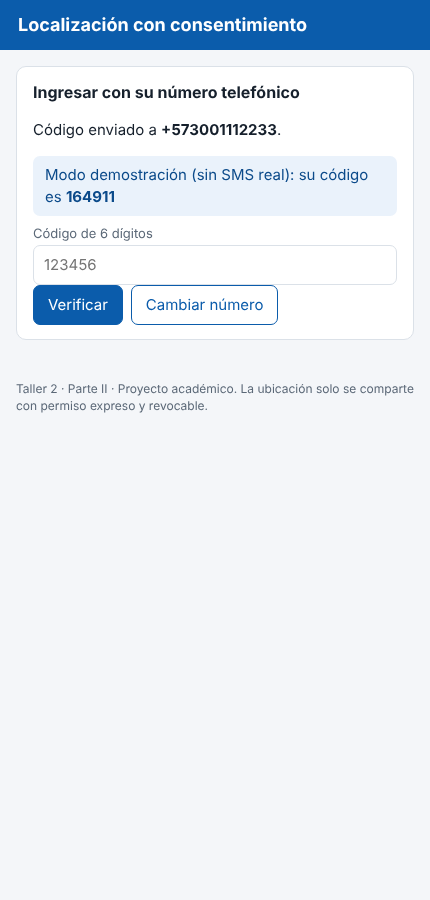
\includegraphics[height=8.6cm]{fig/01-registro-codigo.png}\hspace{0.6cm}
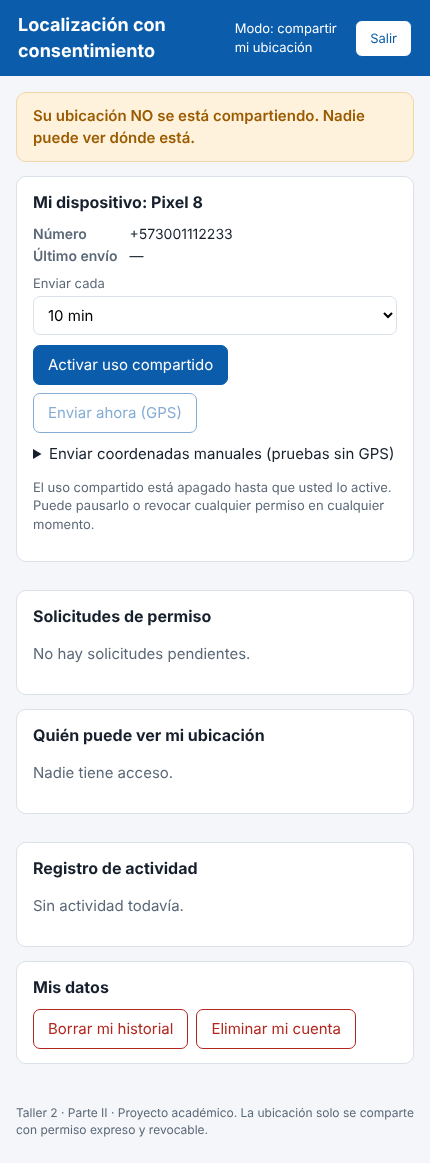
\includegraphics[height=8.6cm]{fig/02-dispositivo-apagado.png}
\caption{Registro por número con código (izquierda; en modo demostración el código se muestra en pantalla porque el SMS es simulado) y estado inicial del titular: la ubicación no se comparte (derecha).}\end{figure}
\fig[0.8]{03-observador-pendiente.png}{El observador pidió permiso: la solicitud queda pendiente y no hay botón de mapa.}
\begin{figure}[H]\centering
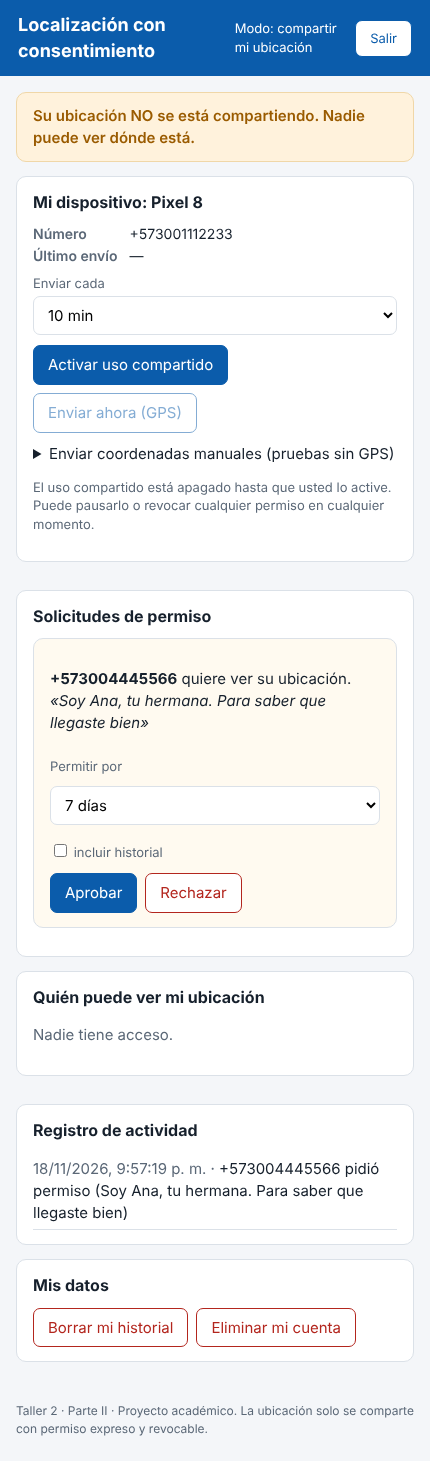
\includegraphics[height=10cm]{fig/04-solicitud-recibida.png}\hspace{0.6cm}
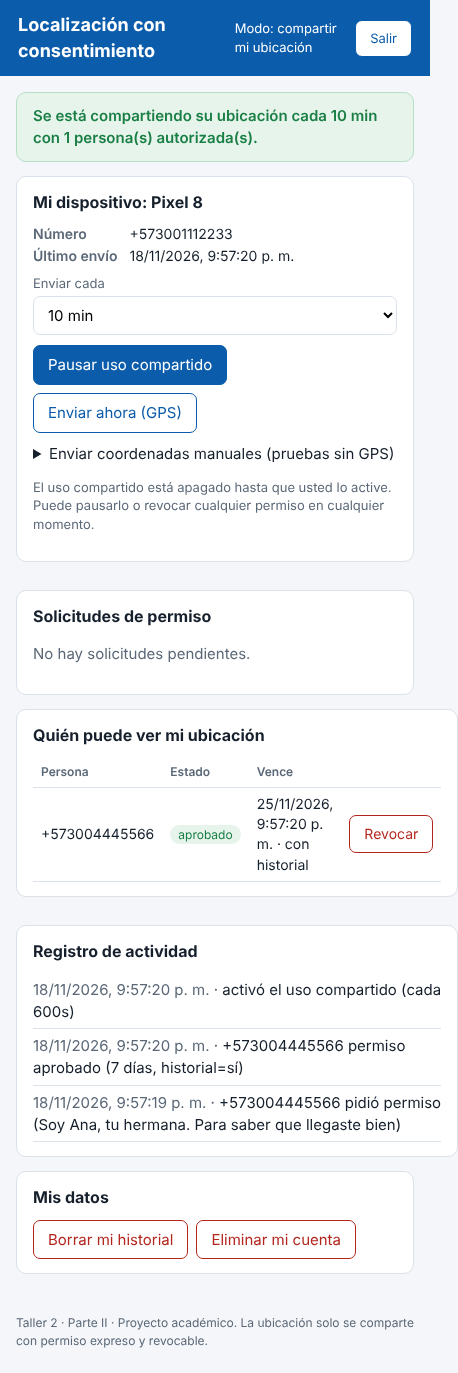
\includegraphics[height=10cm]{fig/05-dispositivo-compartiendo.png}
\caption{El titular recibe la solicitud con el mensaje del observador y elige duración e historial (izquierda). Tras aprobar 7 días con historial y activar el uso compartido, el aviso cambia y el registro de actividad anota cada paso (derecha).}\end{figure}
\fig[0.8]{06-mapa-historial.png}{El observador autorizado ve la última posición, el recorrido y la distancia recorrida.}
\fig[0.8]{07-zona-alerta.png}{Zona ``Casa'' de 300~m y alerta de salida cuando el titular envía una posición a unos 4,6~km.}
\begin{figure}[H]\centering
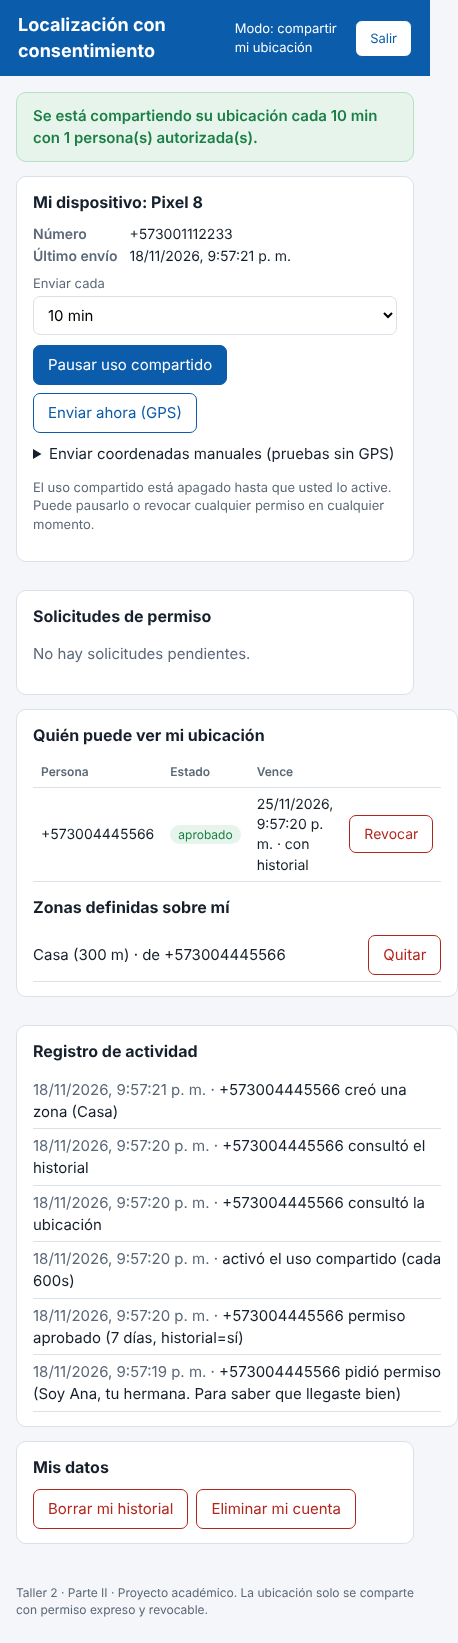
\includegraphics[height=10cm]{fig/08-dueno-registro.png}
\caption{El titular ve quién consultó su ubicación y cuándo, y puede revocar.}\end{figure}
\fig[0.8]{09-acceso-revocado.png}{Tras la revocación, el observador pierde el acceso en la siguiente petición.}

La prueba encontró un fallo real de la interfaz: dos refrescos del mapa en paralelo dibujaban el marcador dos veces. Se corrigió con un contador de secuencia que descarta las respuestas viejas.

\fig[0.98]{term-p2-tests.png}{Las 61 pruebas automáticas de la API: autenticación, consentimiento, ubicaciones, geocercas, retención y borrado.}

\section{Cobertura de requisitos}
\begin{table}[H]\centering\small\caption{Requisitos de la guía y estado.}
\begin{tabularx}{\linewidth}{@{}p{4.6cm}p{1.6cm}X@{}}\toprule
\textbf{Requisito} & \textbf{Estado} & \textbf{Detalle}\\\midrule
Registro por número y verificación por SMS & Parcial & Código de 6 dígitos implementado; envío de SMS simulado (consola), con interfaz para un proveedor real\\
Solicitud y captura de ubicación & Cumplido & GPS del navegador con permiso; envío manual o coordenadas para pruebas\\
Actualización periódica & Cumplido & Intervalo configurable, 10 min por defecto; mientras la página esté abierta\\
Visualización en mapa & Cumplido & Leaflet con OpenStreetMap\\
Historial por fecha y hora & Cumplido & Recorrido y lista con marca de tiempo, si el titular lo permite\\
Alertas por zona (opcional) & Cumplido & Entrada y salida; la primera lectura fija el estado sin alertar\\
Acceso seguro & Cumplido & Token por sesión, permisos por observador\\
API REST y base de datos & Cumplido & FastAPI; SQLite (PostgreSQL, MongoDB y Firebase no se probaron)\\
Geocodificación inversa & Parcial & Implementada, desactivada sin red\\
Estadísticas de movimiento & Cumplido & Puntos y distancia (fórmula de Haversine)\\
Panel web & Cumplido & Interfaz de observador\\
Bot de Telegram (opcional) & No & No implementado\\
Varios dispositivos & No & Un dispositivo por cuenta\\
Ahorro de batería & No & Un navegador no garantiza envíos con la pantalla bloqueada\\
\bottomrule\end{tabularx}\end{table}

\section{Revisión de seguridad del prototipo}
La revisión sigue los controles de autenticación, sesión y validación de OWASP ASVS \cite{owasp} adaptados al riesgo propio de un localizador.
\begin{table}[H]\centering\small\caption{Riesgos y controles implementados.}
\begin{tabularx}{\linewidth}{@{}p{4.2cm}X@{}}\toprule
\textbf{Riesgo} & \textbf{Control}\\\midrule
Seguimiento encubierto & Compartir apagado por defecto; aviso permanente; ver exige aprobación explícita\\
Permiso indefinido & Vence entre 1 y 90 días; el vencimiento se aplica en cada consulta\\
No poder retirar el permiso & Revocación inmediata; el observador pierde acceso en la siguiente petición\\
Consultas ocultas & Registro de actividad visible para el titular\\
Hostigamiento con solicitudes & 5 solicitudes por día por observador; 24~h de espera tras un rechazo\\
Saber si un número usa el sistema & Respuestas idénticas exista o no el número\\
Adivinar el código & 6 dígitos de \cod{secrets}; guardado solo como HMAC-SHA256; 5 intentos; vigencia 10 min; 3 códigos por 10 min por número y 20 por hora por IP\\
Robo de la base de datos & Tokens guardados como SHA-256; nunca en claro\\
XSS & CSP restrictiva; la interfaz no usa \cod{innerHTML}; datos insertados con \cod{textContent}\\
Fuga por caché o referer & \cod{Cache-Control: no-store} en la API; \cod{Referrer-Policy: no-referrer}; \cod{nosniff}\\
Acumulación de datos & Retención de 30 días; borrar historial y eliminar cuenta\\
\bottomrule\end{tabularx}\end{table}

\section{Privacidad y marco legal}
El diseño sigue los principios de la Ley 1581 de 2012: el consentimiento es previo, expreso e informado (el observador explica quién es y para qué, el titular decide); la finalidad y el tiempo están acotados (vencimiento); el acceso está restringido a quien el titular autoriza; y el titular puede conocer (registro de actividad) y suprimir sus datos (borrado). En un despliegue real harían falta además una política de tratamiento publicada, HTTPS obligatorio (la geolocalización del navegador lo exige fuera de \emph{localhost}) y un proveedor de SMS con acuerdo de tratamiento de datos.

\section{Límites}
Es una aplicación web, no nativa; el SMS es simulado; no hay bot de Telegram ni varios dispositivos por cuenta; la base de datos es SQLite; los mosaicos del mapa requieren Internet; y la seguridad se comprobó con pruebas propias, sin auditoría independiente.

\chapter{Discusión y análisis}\label{cap:discusion}

\section{Interpretación de los resultados}
Los diez casos comparten una lección: \textbf{un indicador aislado no confirma un ataque}. Una ráfaga de SYN, una etiqueta DNS de alta entropía, un RST con \emph{ack = 0} o un ping de 1300~B tienen explicaciones legítimas. Lo que convierte un indicador en hallazgo es el contexto: la correlación del saludo TCP, la agrupación por origen y dominio, la tupla de la sesión, la comparación con una línea base medida.

Medir corrige supuestos. Contar SYN no es contar puertos (Caso 8: 25 sondeos, 24 puertos); contar paquetes con ACK no es contar conexiones (Caso 1); el tamaño de trama no es el payload (Caso 7); la media de una captura de 21~s no es la tasa de una ráfaga de 10~s. Por eso todas las cifras salen de scripts que cualquiera puede volver a ejecutar, y la re-ejecución para este informe reprodujo las salidas byte a byte.

La ubicación del control importa tanto como el control. El gateway del laboratorio no reenvía tráfico y no ve lo que circula entre peers de la subred; por eso cada regla propuesta se instala en el host protegido y no en el gateway. En una red real esto equivale a preguntarse siempre si el firewall está en la ruta del tráfico que se quiere filtrar.

\section{Efecto de limpiar la línea base}
La línea base original incluía tráfico ajeno del anfitrión Windows. Se repitieron los casos que la usan sobre la versión limpia (720 paquetes, solo tráfico del laboratorio):

\begin{table}[H]\centering\small\caption{Casos 1, 4 y 7 con la línea base original y con la limpia.}
\begin{tabularx}{\linewidth}{@{}p{3.6cm}p{3.6cm}p{3.6cm}X@{}}\toprule
\textbf{Caso} & \textbf{Original} & \textbf{Limpia} & \textbf{Lectura}\\\midrule
1 SYN flood & 0 SYN en 296,67~s & 0 SYN en 293,26~s & Sin cambio\\
7 ICMP & 152 echo, máx. 1/s, 0 $>$ 200~B & Igual & Sin cambio\\
4 z-score (normales) & 1 falso positivo de 11 & 0 de 11 & Mejora: el error venía del ruido del anfitrión\\
4 Isolation Forest & 5 de 11 & 5 de 11 & Sin cambio\\
4 sintéticas & 22/22 & 22/22 & Sin cambio\\
\bottomrule\end{tabularx}\end{table}

Las conclusiones de los casos 1 y 7 no cambian. En el Caso~4, el único falso positivo del z-score lo causaba el tráfico del anfitrión, lo que muestra cuánto depende un detector de la calidad de su ``normal''. Los resultados están en \cod{evidencia/casos-linea-base-limpia/}, fuera del manifiesto para no alterar la evidencia cerrada.

\section{Límites de la evidencia}
\begin{itemize}
\item Los PCAP de ataque son sintéticos: prueban que el análisis detecta el patrón diseñado, no que funcione ante un atacante real que se adapta.
\item Las reglas nftables se validaron sintácticamente; no se midió su efecto con tráfico.
\item El Caso~4 usa una sola captura de cinco minutos: sus métricas no generalizan.
\item El Caso~9 correlaciona fragmentos de logs de horas distintas; su única alerta es sintética y el dictamen humano está pendiente.
\item Cuatro archivos de texto de la evidencia perdieron sus saltos de línea originales en Git; el manifiesto los registra como enmiendas.
\item Las versiones de herramientas y el uso de un pipeline propio en lugar de Wazuh se asumieron aceptables sin confirmación del docente.
\end{itemize}

\section{Aprendizaje automático y correlación}
Los dos enfoques de detección automática del taller apuntan en la misma dirección: sirven para \textbf{ordenar} la atención del analista, no para decidir. Isolation Forest marcó casi la mitad de las ventanas normales posteriores; un bloqueo automático basado en él cortaría tráfico legítimo con frecuencia. La correlación del Caso~9 es útil precisamente porque cada punto de la alerta se explica y enlaza a la línea de log que lo produjo, de modo que una persona puede verificarla.

\chapter{Conclusiones y trabajo futuro}\label{cap:conclusiones}

\section{Conclusiones}
\begin{enumerate}
\item Se montó un laboratorio aislado, sincronizado y verificable, y se demostró su aislamiento por configuración (sin NAT ni ruta por defecto) y no solo por un ping sin respuesta.
\item Los diez casos se documentaron con fichas uniformes y cifras recalculables. Las salidas se reprodujeron byte a byte y el paquete de entrega verifica 242 archivos por copia.
\item Los controles básicos y bien ubicados —limitar tasa en el host protegido, cerrar servicios innecesarios, exigir y validar TLS, restringir la recursión DNS— reducen más riesgo que cualquier detector sofisticado.
\item El aprendizaje automático y la correlación priorizan la revisión humana. Sus métricas dependen de la calidad de la línea base y de una separación temporal honesta entre entrenamiento y prueba.
\item El sistema de localización demuestra que se pueden cumplir los requisitos funcionales sin sacrificar al titular: permiso por defecto denegado, temporal, revocable y auditable, verificado con 61 pruebas y un recorrido completo en navegador.
\end{enumerate}

\section{Trabajo futuro}
\begin{itemize}
\item Instalar Suricata o Zeek en una VM sensor y ejecutar las reglas propuestas sobre réplicas controladas del tráfico, midiendo su efecto real.
\item Capturar varias líneas base en días distintos para entrenar y validar el Caso~4 con muestras independientes.
\item Completar el dictamen humano del Caso~9 y extender el pipeline con ingestión continua.
\item En la Parte II: proveedor real de SMS, HTTPS con certificado válido, PostgreSQL, bot de Telegram en el que el usuario inicia el chat y comparte su ubicación, y una app nativa para envíos en segundo plano.
\item Emitir certificados desde una CA interna con renovación automática para XMPP y web.
\end{itemize}

\section{Recomendaciones}
\begin{itemize}
\item Conservar siempre la evidencia original con su huella y trabajar sobre copias; fijar en Git que la evidencia se guarde byte a byte desde el primer commit.
\item Capturar la línea base con el anfitrión en silencio o filtrar desde el inicio el tráfico ajeno al laboratorio.
\item Declarar en cada hallazgo qué se probó y qué no; un ``no confirmado'' honesto vale más que una conclusión exagerada.
\end{itemize}

\begin{thebibliography}{99}
\addcontentsline{toc}{chapter}{Referencias}
\bibitem{ieee8023} IEEE, ``IEEE Standard for Ethernet,'' IEEE Std 802.3-2022, 2022.
\bibitem{rfc9293} W. Eddy, ``Transmission Control Protocol (TCP),'' RFC 9293, IETF, 2022.
\bibitem{rfc768} J. Postel, ``User Datagram Protocol,'' RFC 768, IETF, 1980.
\bibitem{rfc792} J. Postel, ``Internet Control Message Protocol,'' RFC 792, IETF, 1981.
\bibitem{rfc1035} P. Mockapetris, ``Domain Names — Implementation and Specification,'' RFC 1035, IETF, 1987.
\bibitem{rfc4987} W. Eddy, ``TCP SYN Flooding Attacks and Common Mitigations,'' RFC 4987, IETF, 2007.
\bibitem{rfc5961} A. Ramaiah, R. Stewart y M. Dalal, ``Improving TCP's Robustness to Blind In-Window Attacks,'' RFC 5961, IETF, 2010.
\bibitem{bcp38} P. Ferguson y D. Senie, ``Network Ingress Filtering: Defeating Denial of Service Attacks which employ IP Source Address Spoofing,'' BCP 38 / RFC 2827, IETF, 2000.
\bibitem{rossow2014} C. Rossow, ``Amplification Hell: Revisiting Network Protocols for DDoS Abuse,'' en \emph{Proc. NDSS}, 2014.
\bibitem{rfc6120} P. Saint-Andre, ``Extensible Messaging and Presence Protocol (XMPP): Core,'' RFC 6120, IETF, 2011.
\bibitem{rfc8446} E. Rescorla, ``The Transport Layer Security (TLS) Protocol Version 1.3,'' RFC 8446, IETF, 2018.
\bibitem{liu2008} F. T. Liu, K. M. Ting y Z.-H. Zhou, ``Isolation Forest,'' en \emph{Proc. IEEE ICDM}, 2008, pp. 413--422.
\bibitem{nist80061} P. Cichonski, T. Millar, T. Grance y K. Scarfone, ``Computer Security Incident Handling Guide,'' NIST SP 800-61 Rev. 2, 2012.
\bibitem{nist80086} K. Kent, S. Chevalier, T. Grance y H. Dang, ``Guide to Integrating Forensic Techniques into Incident Response,'' NIST SP 800-86, 2006.
\bibitem{nftables} Proyecto netfilter, ``nftables wiki: Rate limiting matchings,'' \url{https://wiki.nftables.org}.
\bibitem{ley1581} Congreso de Colombia, Ley Estatutaria 1581 de 2012, por la cual se dictan disposiciones generales para la protección de datos personales.
\bibitem{ley1273} Congreso de Colombia, Ley 1273 de 2009, por medio de la cual se crea el bien jurídico tutelado ``de la protección de la información y de los datos''.
\bibitem{owasp} OWASP Foundation, ``Application Security Verification Standard 4.0.3,'' 2021.
\bibitem{repo} J. E. Buitrago Chavez, repositorio del laboratorio, \url{https://github.com/yatoDx/Laboratorio-seguridad-tcpip}, commit \texttt{bdd8fd6}, 2026.
\end{thebibliography}

\appendix
\chapter{Índice de evidencias e integridad}
Huellas SHA-256 de las capturas, calculadas sobre la rama \cod{main} (commit \cod{bdd8fd6}). Los archivos binarios no dependen de los saltos de línea; para los de texto la referencia es el manifiesto \cod{entrega-parte-i/manifiesto-sha256.json} (SHA-256 \cod{a20e963a47a0ba57\-aff35b1d71616e77\-dfbb8e5032fbae7e\-6f90c897d66af66c}), que cubre 242 archivos por copia y registra las cuatro enmiendas de saltos de línea.

{\small\renewcommand{\arraystretch}{1.2}
\begin{longtable}{@{}p{5cm}p{5.6cm}p{3cm}@{}}
\caption{Capturas de la entrega y su huella SHA-256.}\\\toprule
\textbf{Archivo} & \textbf{Contenido} & \textbf{SHA-256}\\\midrule\endfirsthead
\toprule\textbf{Archivo} & \textbf{Contenido} & \textbf{SHA-256}\\\midrule\endhead
{\ttfamily\scriptsize baseline-normal.pcapng} & Línea base real original (1.639 paquetes) & \cod{\scriptsize 301ea4766c642919\newline 734e3649b1de4c04\newline 9bb4bebeb8ff9b41\newline 25306322b3b076ff}\\
{\ttfamily\scriptsize baseline-normal-limpia.pcapng} & Línea base filtrada al laboratorio (720) & \cod{\scriptsize 6fbe5c7939dfcc5c\newline f254f1bb88d9081e\newline de6ee287e0f91933\newline dbdf602bb66b4427}\\
{\ttfamily\scriptsize caso01-synflood-ratelimit.pcap} & Caso 1, modelo token bucket & \cod{\scriptsize 89875054c5728a4f\newline 5f84e352588a2ca6\newline c1a5e0c17f12c0d5\newline eac753164897865c}\\
{\ttfamily\scriptsize caso01-synflood.pcap} & Caso 1, ráfaga SYN & \cod{\scriptsize cdb0035700ebd5db\newline 641e0908a15331ce\newline ae72148ed3604daa\newline 27f9b7496518de27}\\
{\ttfamily\scriptsize caso02-dns-tunneling.pcap} & Caso 2, consultas DNS & \cod{\scriptsize 4432598be91337ab\newline 04e6749604bfa9a2\newline f16266ae3b264bd3\newline 66d825c185da4988}\\
{\ttfamily\scriptsize caso05-rst.pcap} & Caso 5, RST & \cod{\scriptsize abea3dec5ae31d8f\newline 2f9fa49c6188a8ed\newline 1b0b1bdcedeb1420\newline bfdc422736fb621a}\\
{\ttfamily\scriptsize caso06-reflexion-udp.pcap} & Caso 6, reflexión UDP & \cod{\scriptsize 512bd19bacdcad6d\newline eb19956e7456fd6d\newline 0041713156f14fb2\newline 983d664325822862}\\
{\ttfamily\scriptsize caso07-icmp.pcap} & Caso 7, ICMP & \cod{\scriptsize 1a2fb2b2291ea1cd\newline 7a87b370ca33053b\newline 0693b8526c6c77d0\newline 890a9dbab13a41ac}\\
{\ttfamily\scriptsize caso08-portscan.pcap} & Caso 8, escaneo & \cod{\scriptsize 322d148fe355df3f\newline 13d16b9749cc34e0\newline 58f8a35b2468a010\newline f5eb305a70e7f313}\\
{\ttfamily\scriptsize caso10-xmpp-tls.pcapng} & Caso 10, XMPP/TLS (real) & \cod{\scriptsize 2206664fd9c48ebd\newline 25af51d6407fc2e3\newline 497defde81a66b2f\newline 0e5163214a6e51fa}\\
\bottomrule
\end{longtable}}

\begin{table}[H]\centering\small\caption{Organización de la evidencia en el repositorio.}
\begin{tabularx}{\linewidth}{@{}p{4.8cm}X@{}}\toprule
\textbf{Ruta} & \textbf{Contenido}\\\midrule
{\ttfamily\scriptsize evidencia/} & Verificaciones del montaje, pantallazos, líneas base, \cod{evidencia.log}\\
{\ttfamily\scriptsize evidencia/casos/} & PCAP, análisis, gráficas, logs y capturas de los diez casos; versiones anteriores en \cod{revision-anterior/}\\
{\ttfamily\scriptsize evidencia/casos-linea-base-limpia/} & Casos 1, 4 y 7 repetidos con la línea base limpia (complementaria)\\
\cod{entrega-parte-i/original}, \cod{trabajo} & Copias idénticas de 242 archivos y manifiesto SHA-256\\
{\ttfamily\scriptsize fichas/} & Las diez fichas en Markdown y la plantilla\\
{\ttfamily\scriptsize scripts/} & Generadores, analizadores, pipeline, cierre, reparación y dictamen\\
{\ttfamily\scriptsize parte2/} & Código, pruebas, documentación y capturas de la Parte II\\
\bottomrule\end{tabularx}\end{table}

\chapter{Reproducción}
Desde la raíz del repositorio, con Python 3, \cod{tshark} y las dependencias de \cod{parte2/requirements.txt}:
\begin{lstlisting}
# integridad del paquete de la Parte I
python3 scripts/cerrar_parte_i.py --verificar
# todas las pruebas (Parte I: 34; Parte II: 61)
./ejecutar_pruebas.sh
# autopruebas del Caso 4 (19)
python3 scripts/caso04_ml.py --self-test
# re-ejecutar un análisis (no transmite tráfico; solo lee PCAP)
python3 scripts/analizar_caso01.py
# Parte II en modo demostración
cd parte2 && LOC_DEV_SHOW_CODE=1 uvicorn app.main:create_app --factory --port 8000
# recorrido completo en Chrome con capturas
python3 tests/e2e_navegador.py
\end{lstlisting}
Los scripts que acceden a las VMs leen el usuario y la contraseña de las variables \cod{LAB\_USER} y \cod{LAB\_PASS}; la contraseña no está en el código actual (versiones anteriores del historial de Git sí la contienen y corresponden a un usuario desechable de la red aislada).

\chapter{Problemas encontrados y soluciones}
\begin{longtable}{@{}p{5cm}p{9.2cm}@{}}
\caption{Problemas encontrados durante el trabajo y cómo se resolvieron.}\\\toprule
\textbf{Problema} & \textbf{Solución}\\\midrule\endfirsthead
\toprule\textbf{Problema} & \textbf{Solución}\\\midrule\endhead
Las VMs necesitaban paquetes pero el laboratorio debía quedar aislado & NAT solo durante la instalación; después \cod{--nic1 none}, netplan limpio y snapshots \cod{lab-base-aislado-v2}\\
La evidencia de NTP de los clientes no aparecía con \cod{timedatectl} & Las VMs usan chrony (heredado de la plantilla); se documentó con \cod{chronyc sources} y \cod{tracking}\\
Claves SSH de host repetidas en las VMs clonadas & Se regeneraron para que cada VM tenga huella propia\\
La línea base contenía tráfico ajeno del anfitrión & Versión limpia filtrada a 192.168.50.0/24 y repetición de los casos 1, 4 y 7\\
Primera versión del Caso 4 con ventanas desiguales y evaluación sobre datos de entrenamiento & Rehecha con ventanas de 10~s, separación temporal, embargo y métricas solo sobre prueba\\
Prosody sin certificado; la recarga no activó el nuevo VirtualHost & Certificado con SAN correcto y reinicio del servicio; el registro conserva la orden original\\
Pseudofirmas de IDS incorrectas (\cod{byte\_test} sobre nombres DNS, \cod{ack:0} como RST forjado) & Retiradas; detección en Python con límites declarados\\
Reglas con \cod{policy drop} general que podían romper servicios & Tablas independientes con política \emph{accept} que solo actúan sobre el exceso, ubicadas en el host protegido\\
El manifiesto no verificaba en un clon por la conversión CRLF/LF de Git & \cod{.gitattributes}, restauración de CRLF y registro de cuatro enmiendas; verificación correcta en clon limpio\\
Contraseña del laboratorio escrita en \cod{vmctl.py} & Lectura desde \cod{LAB\_PASS}\\
\cod{pytest} en la raíz chocaba con las copias de \cod{entrega-parte-i} & \cod{pytest.ini} y \cod{ejecutar\_pruebas.sh}\\
Marcador duplicado en el mapa de la Parte II & Contador de secuencia que descarta respuestas viejas\\
Wireshark instalado pero fuera del PATH & El verificador lo busca en su carpeta de instalación\\
\bottomrule
\end{longtable}

\end{document}
